% !TEX program = lualatex
\documentclass[UTF8, a4paper, 12pt]{ctexart}

%% === 导言区：宏包配置 ===
\usepackage{geometry}
\geometry{left=2.5cm,right=2.5cm,top=2.5cm,bottom=2.5cm} % 标准页边距
\usepackage{amsmath, amssymb,amsthm} % 数学公式
\newtheorem{proposition}{命题}
\newtheorem{remark}{注}
\newtheorem{definition}{定义}
\newtheorem{theorem}{定理}
\usepackage{graphicx}         % 图片支持
\usepackage{array}
\usepackage{tabularx}
\usepackage{booktabs}     
\usepackage{enumitem}    % 顶刊必备：专业三线表
\usepackage{algorithm}        % 算法环境
\usepackage{algorithmic}      % 算法伪代码
\usepackage{longtable}        % 允许表格跨页
\usepackage{multirow}         % 表格多行合并
\usepackage{makecell}         % 单元格内换行
\usepackage{threeparttable}   % 表格注释环境
\usepackage{subcaption}       % 子图
\usepackage{placeins}         % 防止浮动体越过参考文献
\usepackage{calc}              % 尺寸计算（用于图片占位框）
\usepackage[table]{xcolor}    % 表格颜色高亮 (必须加 table 选项)
\usepackage{hyperref}         % 超链接
\hypersetup{
    colorlinks=true,
    linkcolor=black,
    citecolor=blue,           % 引用显示为蓝色，方便审稿人查看
    urlcolor=blue
}

% 投稿版排版微调
\captionsetup{font=small,labelfont=bf}
\captionsetup[figure]{skip=6pt}
\captionsetup[table]{skip=4pt}
\setcounter{topnumber}{3}
\setcounter{bottomnumber}{2}
\setcounter{totalnumber}{5}
\renewcommand{\topfraction}{0.9}
\renewcommand{\bottomfraction}{0.8}
\renewcommand{\textfraction}{0.07}
\clubpenalty=10000
\widowpenalty=10000
\displaywidowpenalty=10000

%% === 正文开始 ===
\begin{document}

%% --- 标题页 ---
% 标题
\title{\heiti\zihao{2} 考虑并行作业掩盖效应的靠泊船舶异质能源服务调度优化}
\author{}
\date{}
\maketitle

\begin{abstract}
在港口绿色转型加速推进的背景下，靠泊船舶的能源服务已由单一岸电供给演化为岸电、换电与传统燃油辅机并存的异质补能系统。现有相关研究多采用“先装卸、后补能”的串行作业假设，且通常仅刻画单一能源模式，因而难以识别并行作业（SIMOPS）对船舶停港时间和系统成本结构的真实影响。本文围绕港口异质能源服务调度问题，构建了一个显式刻画 SIMOPS 掩盖效应的统一优化框架：当能源服务在装卸窗口内完成时，其时间消耗不再线性增加船舶停港时长，而由装卸作业与补能作业的最大完工时刻共同决定离港时间。基于此，本文建立了时间展开的混合整数规划模型，并设计了基于列生成与整数恢复的求解框架，以应对大规模实例下直接求解 MILP 的计算瓶颈。

修正后的数值实验表明：在可有效验证的规模上，CG 在 $N=20$ 和 $N=50$ 时与精确 MILP 基准一致；当规模增至 $N=100$ 时，限时 MILP 已难以提供稳定基准，而 CG 仍保持 100\% 成功率；在扩大迭代预算后，CG 在 $N=200$ 和 $N=500$ 下仍分别以 120.65s 和 275.90s 的平均时间稳定给出当前实验组中最优的平均结果，并整体优于 Rolling-Horizon、Fix-and-Optimize、Restricted-CG、FIFO 与 Greedy 等对比算法。进一步的场景、SIMOPS、敏感性与机制实验显示：SIMOPS 的收益具有显著的容量条件性；混合补能机制显著优于任何单一补能方案；岸电容量扩张对系统成本和绿色服务结构的改善强于单纯的价格调节。上述结果为港口异质能源基础设施的协同规划与运行调度提供了更具解释力和工程可操作性的定量依据。
\end{abstract}

\noindent\textbf{关键词：}港口调度；并行作业（SIMOPS）；岸电；电池换电；列生成

%% --- 第一章：绪论 ---
\section{绪论}
\label{sec:intro}

\subsection{研究背景与动机}
在国际海事组织（International Maritime Organization, IMO）日益严格的环境监管框架下，全球航运业正面临深度脱碳转型的迫切需求。船舶在港期间由辅助柴油发电机产生的污染排放，已成为港口碳减排治理中的重点对象。为此，岸电（Shore Power, SP）与电池换电（Battery Swapping, BS）已逐渐成为绿色港口建设中两类具有代表性的船舶补能技术路径。
 
岸电技术依托港口固定供电设施，为靠泊船舶直接供电，具有能源成本低、技术成熟度高等优势。如图~\ref{fig:realworld_motivation} 左图所示，集装箱船靠泊后，岸电电缆通过标准化接口连接至船舶配电系统，在货物装卸作业期间同步为船载设备持续供电——这一"供电与装卸并行"的操作模式已被 IEC/IEEE~80005-1 国际标准 \cite{IEC80005} 确立为规范化作业流程。在国际层面，鹿特丹港作为欧洲最大集装箱枢纽（年吞吐量约 1,500 万 TEU），已在 ECT Delta 等主要集装箱码头部署岸电系统，并与安特卫普港、汉堡港等签署联合备忘录，承诺在欧盟《FuelEU 海事法规》\cite{EU2025} 要求的 2030 年截止日期前实现岸电全面覆盖 \cite{Winkel2016}；届时，所有靠泊欧盟港口的集装箱船将被强制要求使用岸电，这使得岸电容量的高效调度成为港口运营的核心挑战。在长江流域，宜昌港已率先实现大规模岸电部署：截至 2025 年初，宜昌段 63 个经营性码头全面覆盖岸电服务，建成投运岸电桩 172 台，累计为逾 48{,}000 艘次船舶提供清洁岸电 \cite{ICCT2023}。然而，无论是鹿特丹的欧洲枢纽港还是宜昌的内河大港，岸电的接入与充电过程通常耗时较长（单船充电时间可达数小时），并受泊位及电力基础设施容量的严格约束，在船舶密集到港时容易形成排队等待。
 
电池换电技术则提供了截然不同的补能路径。如图~\ref{fig:realworld_motivation} 右图所示，移动换电设备通过起重机械快速更换船载整组电池，整个过程通常可在 45 分钟至 2 小时内完成 \cite{Zhang2022_EShip}。以宜昌—武汉航线为例，全国首艘长江支线换电集装箱船"华航新能1"号已在宜昌港域商业运营，实现在靠港期间完成整组电池更换并立即离港，与传统岸电充电模式形成显著的时间互补。值得注意的是，宜昌港在推进岸电全覆盖的同时，正是上述换电集装箱船的运营母港——这意味着两类补能基础设施已在同一港域内共存，并分别服务于不同时间敏感程度的船舶，但目前尚无统一的联合调度框架对二者进行协同优化。与岸电相比，换电模式在时间效率上具有显著优势，但伴随较高的服务费用和对港口电池库存管理能力的要求。
 
\begin{figure}[!htbp]
    \centering
    \begin{subfigure}[b]{0.48\textwidth}
        \centering
        \includegraphics[width=\textwidth,height=5cm,keepaspectratio]{ltd.jpg}
        \caption{岸电连接现场（鹿特丹港/宜昌港）\\（装卸期间同步供电；欧盟 2030 年强制部署，宜昌已全覆盖）}
        \label{fig:ltd.jpg}
    \end{subfigure}
    \hfill
    \begin{subfigure}[b]{0.48\textwidth}
        \centering
        \includegraphics[width=\textwidth,height=5cm,keepaspectratio]{cjhd.jpg}
        \caption{换电集装箱船靠港作业（宜昌—武汉航线）\\（"华航新能1"号换电作业，45 分钟至 2 小时完成补能）}
        \label{fig:realworld_bs}
    \end{subfigure}
    \caption{\textbf{两类补能技术的工程实践——以宜昌港为汇聚点。}
    (a) 岸电技术在国际与国内港口均已大规模部署：鹿特丹港已在主要集装箱码头建成岸电系统，欧盟法规要求 2030 年强制推广；宜昌港已实现辖区 63 个码头岸电全覆盖。船舶靠泊后，岸电连接可贯穿装卸作业全程（SIMOPS），已由 IEC/IEEE 80005-1 标准规范化。
    (b) 换电技术已在宜昌—武汉航线的"华航新能1"号等长江换电集装箱船上商业运营：移动换电设备可在约 45 分钟至 2 小时内完成整组电池更换，为时间敏感型船舶提供快速离港选项。
    两类设施已在宜昌港域内同时部署，分别服务于不同补能需求的船舶；如何在允许两类服务并存的港口中进行联合调度优化，正是本文研究的核心问题。}
    \label{fig:realworld_motivation}
\end{figure}
% 注：投稿时请将占位框替换为真实照片。推荐图片来源：
% (a) 鹿特丹港官网 / IMO 绿色港口报告 / IRENA 可再生能源港口报告
% (b) 长江三峡集团新闻 / 工信部电动船舶示范项目报告 / 宜昌换电船项目
% 确保获得使用授权或选用公开版权（CC）图片
 
由于两种补能模式在时间效率与成本结构上的互补特性，现实港口运行中正逐渐形成岸电与换电并存的混合服务格局：时间敏感型船舶（如冷藏集装箱船、快速周转支线船）倾向于选择换电以快速离港，而时间充裕的船舶则优先使用低成本岸电。这种异质性服务需求为港口能源调度带来了新的复杂性。
 
在政策和市场的双重驱动下，港口侧多元电气化需求正在国际范围内快速形成。在需求侧，全球电动船舶市场预计将在 2025 年至 2030 年间以超过 20\% 的年复合增长率（CAGR）迅速扩张 \cite{Markets2025}，催生出岸电与换电并存的异质性港口服务格局。在政策供给侧，欧盟《FuelEU 海事法规》明确强制要求集装箱船和客船在 2030 年前接入岸电 \cite{EU2025}，使鹿特丹、安特卫普等欧洲主要港口面临在有限泊位资源下同时满足大规模岸电接入需求的调度压力；与此同时，中国交通运输部在长江经济带积极推进换电基础设施建设，并将宜昌作为"电化长江"核心示范区，推动岸电与换电在同一港域内的规模化并行部署。上述政策趋势表明，如何对异质能源服务进行统一调度，已成为当前国际港口运营的共性挑战，而非局限于特定港口或地区的个例。
 
然而，现有港口运营优化研究在刻画能源补给与装卸作业的协同关系方面仍存在明显不足。多数文献要么聚焦于单一能源资源的配置与调度，要么将能源补给视为独立于核心装卸作业之外的附加环节，忽视了两类作业在时间维度上的潜在重叠关系。更重要的是，如图~\ref{fig:realworld_motivation}(a) 所示，岸电连接实际上在货物装卸窗口内同步进行——若建模时将两者串行叠加，将系统性高估船舶在港停留时间，从而扭曲资源配置与调度决策。此外，在船舶数量增加、运行环境动态化的背景下，传统精确优化方法在大规模实例下的计算效率局限性日益凸显，难以满足实时决策需求。
\subsection{文献综述}
\label{sec:lit_review}
 
本节从泊位分配问题的基础研究、港口岸电资源配置与泊位联合调度、电动船舶换电模式与移动补能优化，以及异质性能源协同与并行作业机制四个维度，对现有相关研究进行系统回顾，并指出现有文献的局限性，从而确立本文的研究定位。
 
\subsubsection{泊位分配问题研究进展}
 
泊位分配问题（Berth Allocation Problem, BAP）是港口运营优化研究的基础性问题。
Lim (1998) \cite{Lim1998} 最早将 BAP 形式化为图论框架，证明其属于 NP 难问题，奠定了该领域的计算复杂性认知。
Imai 等 (2001) \cite{Imai2001} 建立了动态 BAP 的整数规划模型，将船舶到达的随机性显式纳入调度框架，首次揭示了动态负载对泊位利用率的系统性影响。
Bierwirth 与 Meisel (2010) \cite{Bierwirth2010} 在首次综述中系统梳理了 BAP 与岸桥调度问题（QCSP）的研究脉络，将问题按空间模型（离散/连续）和时间模型（静态/动态）进行分类，为后续研究提供了统一框架。
在精确求解方面，Correcher 等 (2019) \cite{Correcher2019} 提出了针对连续 BAP 的分支定价算法，通过列生成分解将大规模实例的求解时间压缩至可接受范围，为本文的算法设计提供了方法论参照。
Rodrigues 与 Agra (2022) \cite{Rodrigues2022} 在最新综述中总结指出，随着港口电气化需求的增长，BAP 的约束集合正逐步扩展至能源供给、碳排放等环境维度，传统仅考虑空间与时间的建模框架已难以完整刻画现代港口的运营复杂性。
 
上述研究构成本文建模的基础背景。本文在继承 BAP 的时间窗与资源竞争建模范式的同时，进一步将能源服务选择与 SIMOPS 并行作业机制引入调度框架，对传统 BAP 研究体系进行扩展。
 
\subsubsection{港口岸电资源配置与泊位联合调度}
 
岸电（Shore Power, SP）作为降低船舶在港排放的成熟技术，其调度优化是绿色港口研究的持续热点。
Winkel 等 (2016) \cite{Winkel2016} 对欧洲主要港口的岸电基础设施部署现状进行了系统评估，指出岸电接口的容量配置是制约绿色港口建设的主要瓶颈，并建议在泊位规划阶段即纳入岸电资源约束。
Zis 等 (2014) \cite{Zis2014} 通过定量比较岸电接入与航速优化两类减排措施，发现在靠泊时间较长的干线航线上，岸电接入的单位减排成本显著低于航速调整，为政策层面推广岸电提供了经济学依据。
Iris 与 Lam (2019) \cite{Iris2019} 在港口能效综述中进一步指出，岸电调度与泊位分配的解耦处理会系统性低估资源冲突频率，建议在港口能源管理系统中推行联合优化。
在联合调度建模方面，Dai 等 (2020) \cite{Dai2020} 较早提出了岸电泊位分配问题（BAP-SP），目标是在最小化碳排放的同时最大化岸电桩的利用率。Wang 等 (2024) \cite{Wang2024_SP} 进一步引入多目标优化框架，利用 NSGA-III 算法协同优化泊位调度与岸电分配，证明了联合调度能显著降低船舶的在港等待时间。Zou 等 (2024) \cite{Zou2024} 则在考虑电网负荷波动的条件下建立了岸电动态定价与泊位分配联动模型，揭示了电价不确定性对绿色能源占比的抑制效应。
 
然而，上述研究普遍将岸电视为唯一清洁能源来源，忽略了日益增长的移动补能需求，难以应对异质能源并存的复杂运营场景。
 
\subsubsection{电动船舶换电模式与移动补能优化}
 
与岸电的固定基础设施属性不同，电池换电（Battery Swapping, BS）为航运业提供了"以成本换时间"的灵活补能路径。
Wu 等 (2020) \cite{Zhang2022_EShip} 在系统综述中指出，换电技术特别适用于内河及短途海运场景，其核心优势在于将能量补给时间从小时级压缩至分钟级，同时将电池管理与充电基础设施从船端转移至岸端。
Bei 与 Li (2024) \cite{Bei2024} 建立了内河电动船队的换电站选址—容量联合规划模型，证明在航线密度较高的内河走廊，换电站网络的投资回报率显著优于岸上充电模式。
Zhang 等 (2024) \cite{Zhang2024_Voyage} 针对内河全电动船队提出了基于换电站布局的航次调度模型，验证了换电模式在提升船队周转效率方面的优势。
Li 等 (2022) \cite{Li2022_BSS} 则从电网互动角度研究了换电站的充放电策略以响应分时电价信号，发现"谷电充电、峰时待命"的策略可将换电站运营成本降低约 15\%--25\%。
道路交通领域的换电调度研究提供了重要的方法论参照。Mak 等 (2013) \cite{Mak2013} 针对电动汽车换电网络建立了鲁棒基础设施规划模型，所提出的容量约束下排队服务框架与本文换电容量约束的建模思路具有结构相似性。
 
然而，上述研究大多将换电视角局限于单一补能网络或内河航运，尚未将移动换电资源与岸电、燃油等多类服务整合进统一的大规模集装箱码头调度框架。
 
\subsubsection{异质性能源协同与并行作业机制}
 
在实际港口运营中，岸电（固定、廉价、长时）与换电（移动、昂贵、短时）在技术特征上具有天然的互补性，但现有港口调度文献鲜有将二者纳入统一框架。
Yang 等 (2025) \cite{Zhen2022_SP} 建立了混合动力拖轮的岸电与燃油联合调度模型，证明动态能源切换策略可显著降低辅助作业船只的综合运营成本，然而其研究对象仅限于辅助作业船只，且未考虑货物装卸对能源服务时间窗的约束，难以直接推广至集装箱码头场景。
Psaraftis (2019) \cite{Psaraftis2019} 与 Wang 等 (2023) \cite{Wang2023} 的研究从更宏观的视角指出，碳税与绿色物流政策将系统性重塑港口能源服务的成本结构，推动异质补能方案的经济可行性进入新的阈值区间。
 
更关键的是，包括上述文献在内的现有研究均隐含地采用\emph{串行作业假设}：能源补给须在装卸完成后方可进行。这一假设与工程实践存在根本性偏差。
在 LNG 加注领域，Fan 等 (2021) \cite{Fan2021} 通过定量风险评估证实，并行作业（SIMOPS）不仅在 OCIMF 与 SIGTTO 安全规范框架内可行，而且是提升港口效率的关键操作手段，其风险水平完全在可接受范围之内。
Br\"{o}ckmann 等 (2022) \cite{Fan2022_SIMOPS} 进一步分析了 LNG 加注与货物装卸并行作业的风险控制规程，指出在完备的操作程序与实时监控条件下，SIMOPS 所带来的安全附加风险可被有效管控。
在岸电领域，IEC/IEEE~80005-1 国际标准 \cite{IEC80005} 明确规定，岸电连接流程可在船舶完成系缆后立即启动，并贯穿货物装卸的全过程，从而在技术标准层面为 SIMOPS 提供了规范性依据。
Notteboom (2006) \cite{Notteboom2006} 通过分析班轮运输中时间成本的经济权重，从供应链视角论证了并行作业对缩短在港时间、降低全程运输成本的战略意义。
 
然而，尽管 SIMOPS 在工程实践中已被广泛采用，至今尚无研究将其并行机制数学化地引入大规模集装箱码头的异质能源协同调度优化模型。这一空白构成本文的核心研究动机。
 
\textbf{研究空白总结：}如表~\ref{tab:lit_review} 所示，现有文献在以下三个维度均存在明显缺口：(i) 异质能源（岸电+换电+燃油）的统一调度框架；(ii) SIMOPS 并行作业机制的数学化建模；(iii) 面向大规模实例的精确求解方法。本文正是为了在单一框架内同时填补上述三项空白而展开研究。
 
\subsection{并行作业掩盖效应与本文定位}
 
基于上一节的文献梳理，本文提出作业掩盖效应（Masking Effect）这一核心概念，并将其纳入港口能源调度的优化框架。
 
\paragraph{掩盖效应的定义}
在允许 SIMOPS 的条件下，只要能源补给作业能够在装卸作业窗口内完成，其时间消耗便不会对船舶总体在港停留时间产生额外影响。此时，船舶在港停留时长由装卸时间与补能时间二者的\emph{较大值}决定，而非两者之和：
\begin{equation*}
\begin{aligned}
T_{\text{stay}} &= \max\{T_{\text{cargo}},\; T_{\text{energy}}\} + W_{\text{queue}}
&& \text{（并行作业）} \\
T_{\text{stay}} &= T_{\text{cargo}} + T_{\text{energy}} + W_{\text{queue}}
&& \text{（串行作业）}
\end{aligned}
\end{equation*}
本文将并行作业引发的时间折扣现象称为\emph{作业掩盖效应}。需要强调的是，SIMOPS 并非理论假设，而是海事工业界为应对紧张船期而广泛采用的标准操作流程，其工程实践基础已在第~\ref{sec:intro}节图~\ref{fig:realworld_motivation} 中直观展示。
 
\paragraph{SIMOPS 的约束性}
SIMOPS 并不意味着无约束的完全并行。其可行性受到设备兼容性、安全规范及船舶内部作业冲突等因素的制约。本文在建模过程中显式刻画这些约束，在保证物理可行性的前提下引入掩盖效应。
 
基于上述分析，表~\ref{tab:lit_review} 将本文与现有相关研究在研究对象、能源模式、作业逻辑和求解能力等维度进行系统比较。
 
%% --- 文献对比表 ---
\begin{table}[htbp]
    \centering
    \caption{本文与现有港口能源调度相关研究的特征对比分析}
    \label{tab:lit_review}
    \footnotesize
    \renewcommand{\arraystretch}{1.4}
    \begin{threeparttable}
        \resizebox{\textwidth}{!}{%
        \begin{tabular}{l c c c c c c}
            \toprule
            \textbf{文献来源} & \textbf{研究对象} & \textbf{能源模式} & \textbf{作业逻辑} & \textbf{求解方法} & \textbf{计算规模} & \textbf{异质协同} \\
            \midrule
            \multicolumn{7}{l}{\textit{泊位分配基础研究}} \\
            Lim (1998) \cite{Lim1998}                      & 集装箱码头 & 无能源          & 串行 (Seq.) & 图论/精确  & 小规模   & $\times$ \\
            Imai et al. (2001) \cite{Imai2001}             & 集装箱码头 & 无能源          & 串行 (Seq.) & 整数规划   & 中等     & $\times$ \\
            Correcher et al. (2019) \cite{Correcher2019}   & 集装箱码头 & 无能源          & 串行 (Seq.) & 分支定价   & 高       & $\times$ \\
            \midrule
            \multicolumn{7}{l}{\textit{港口岸电配置与调度}} \\
            Zis et al. (2014) \cite{Zis2014}               & 干线航运   & 仅岸电 (SP)     & 串行 (Seq.) & 情景分析   & —        & $\times$ \\
            Dai et al. (2020) \cite{Dai2020}               & 集装箱码头 & 仅岸电 (SP)     & 串行 (Seq.) & 精确算法   & 中小规模  & $\times$ \\
            Wang et al. (2024) \cite{Wang2024_SP}          & 集装箱码头 & 仅岸电 (SP)     & 串行 (Seq.) & NSGA-III   & 中等     & $\times$ \\
            Zou et al. (2024) \cite{Zou2024}               & 集装箱码头 & 仅岸电 (SP)     & 串行 (Seq.) & 精确算法   & 中等     & $\times$ \\
            \midrule
            \multicolumn{7}{l}{\textit{换电调度与移动补能}} \\
            Mak et al. (2013) \cite{Mak2013}               & 道路交通   & 仅换电 (BS)     & 串行 (Seq.) & 鲁棒优化   & 中等     & $\times$ \\
            Zhang et al. (2024) \cite{Zhang2024_Voyage}    & 内河航运   & 仅换电 (BS)     & 串行 (Seq.) & 启发式     & 中等     & $\times$ \\
            \midrule
            \multicolumn{7}{l}{\textit{异质能源协同与并行作业}} \\
            Yang et al. (2025) \cite{Zhen2022_SP}      & 拖轮调度   & 岸电+燃油       & 串行 (Seq.) & 精确算法   & 小规模   & 部分 \\
            Fan et al. (2021) \cite{Fan2021}               & LNG加注    & 单一能源        & \textbf{并行 (SIMOPS)} & 风险评估 & —  & $\times$ \\
            Br\"{o}ckmann et al. (2022) \cite{Fan2022_SIMOPS} & LNG加注  & 单一能源        & \textbf{并行 (SIMOPS)} & 安全分析 & —  & $\times$ \\
            \midrule
            \rowcolor{gray!15}
            \textbf{本文 (Ours)} & \textbf{集装箱码头} & \textbf{岸电+换电+燃油} & \textbf{并行 (SIMOPS)} & \textbf{列生成+整数恢复} & \textbf{高 ($N$$\le$500)} & \checkmark \\
            \bottomrule
        \end{tabular}%
        }
        \begin{tablenotes}
        \footnotesize
        \item 注：``异质协同'' 列表示研究是否同时考虑多种异质能源服务的统一调度框架。
        \end{tablenotes}
    \end{threeparttable}
\end{table}
 
如表~\ref{tab:lit_review} 所示，现有港口能源调度研究尚无文献同时具备异质能源协同、SIMOPS 并行作业建模与大规模高效求解三项特征。本文正是从这一空白出发，构建统一的港口能源—作业协同调度优化框架。
 

\subsection{算法挑战：打破计算瓶颈}
在大规模动态港口环境中对 SIMOPS 进行建模，引入了复杂的时空耦合约束。虽然精确算法（如分支定价法 B\&P）理论上能找到最优解，但其搜索空间随船舶数量呈指数级增长，在大规模实例中往往面临严峻的计算瓶颈。

正如 Bierwirth 与 Meisel (2015) \cite{Bierwirth2015} 以及 Rodrigues 与 Agra (2022) \cite{Rodrigues2022} 在泊位调度综述中所总结的，BAP 及其扩展问题属于 NP 难问题，即便借助商业求解器，中大规模实例的求解时间仍往往超过可接受范围。这种计算延迟使得精确算法难以直接应用于具有随机到达、滚动决策特征的实际港口运行环境。为缓解计算压力，部分文献转而采用启发式或元启发式方法，但此类方法通常无法提供最优性保证，且对参数调节和问题规模较为敏感。

上述困境反映了港口与运输调度领域中一个更为普遍的方法论挑战：如何在满足实时响应需求的前提下，兼顾计算效率与解的最优性。针对这一问题，本文在保持精确优化框架的基础上，采用列生成（Column Generation, CG）分解思想缓解计算瓶颈，以提升大规模实例下的求解效率。

\subsection{本文贡献}
围绕“异质能源服务选择、SIMOPS 并行作业与大规模精确求解”这一组合问题，本文的主要贡献可归纳为三个方面。

第一，本文在建模层面提出了一个面向港口异质补能系统的统一优化框架。该框架同时刻画岸电、换电与燃油辅机三类服务模式，并将 SIMOPS 由工程操作规则转化为可优化的时间耦合约束，使船舶离港时间由串行加法结构转化为最大值结构，从而能够显式识别装卸窗口对补能时间的掩盖作用及其失效边界。

第二，本文在算法层面构建了基于列生成与整数恢复的分解求解框架。该方法在可处理实例上能够与精确 MILP 基准对齐，并在中大规模实例上保持更好的可扩展性。与直接 MILP 相比，所提方法在保留精确优化逻辑的同时显著缓解了时间展开模型带来的计算压力；与 Rolling-Horizon、Fix-and-Optimize 和 Restricted-CG 等近似优化框架相比，完整 CG 在解质量与规模鲁棒性之间提供了更强的整体平衡。

第三，本文在实证层面系统揭示了港口异质能源调度中的若干关键规律。实验结果不仅验证了所提模型与算法的有效性，也表明：峰值到达比装卸时长整体拉长更易诱发系统拥堵；SIMOPS 的收益取决于容量是否足以支撑并行化需求；混合补能机制显著优于任何单一补能方案；岸电容量扩张相较价格调节具有更强的结构性改善作用。上述发现为港口绿色基础设施投资与运行策略设计提供了直接的管理启示。
%% ==============================================================
%% SECTION 2: PROBLEM DESCRIPTION AND MODEL
%% ==============================================================

%% ==============================================================
%% SECTION 2: PROBLEM DESCRIPTION AND MODEL (FINAL ACADEMIC VERSION)
%% ==============================================================

%% ==============================================================
%% SECTION 2: PROBLEM DESCRIPTION AND MODEL (NARRATIVE FLOW VERSION)
%% ==============================================================

\section{问题描述与数学建模}
\label{sec:model}

\subsection{问题定义与决策结构}
\label{sec:problem_definition_cn}

本文研究的是自动化集装箱码头环境下的港口能源—作业协同调度问题。在船舶靠泊期间，港口运营方需要在满足装卸作业需求的同时，为船舶提供能源服务，并合理协调能源服务选择、资源占用以及船舶离港时序，其目标是最小化包含能源成本、碳排放外部性以及时间机会成本在内的广义运营成本。

从运筹优化的角度来看，该问题可被抽象为一类具有\emph{异质性服务选项}和\emph{异质性延误惩罚}的港口调度问题。在该问题中，能源补给不再被视为独立于装卸作业之外的附属环节，而是与船舶在港停留时间直接耦合的关键决策变量。这一建模视角与近年来将港口视为综合物流—能源系统的研究趋势一致 \cite{andersson2017shipping,bergqvist2019ports}。

在所考虑的系统中，港口运营中心（Terminal Operating Center, TOC）在船舶到达港口后，需要在多个可行的能源服务选项之间为其做出选择，并同时确定能源服务的开始时刻。该决策过程受到港口能源基础设施容量约束、船舶作业时间窗以及船舶对离港延误的异质性敏感程度等多重因素的共同影响。

与大量现有港口与运输调度文献不同，本文允许能源服务与货物装卸作业在时间维度上发生重叠。现有研究普遍采用串行作业假设，即认为船舶必须在完成装卸作业后才能开始能源补给。尽管该假设在建模上较为简洁，但已有研究指出，其可能系统性高估船舶在港停留时间，从而影响资源配置与调度决策的合理性 \cite{Zou2024}。

从问题结构上看，本文研究的是一个\emph{服务选择—排队—离港时序联合优化问题}，其主要特征体现在以下几个方面。

能源服务选项在资源占用方式、服务持续时间以及成本结构方面具有显著的结构异质性。这使得港口能源调度问题不同于传统的单资源或单机器调度问题，而更接近于具有多种服务类型和容量约束的调度问题 \cite{brucker2007scheduling}。图~\ref{fig:scenario} 显示，在港口能源系统中，岸电服务依赖固定泊位和电力基础设施，换电服务依赖移动设备，而传统燃油模式则不消耗任何港口外部资源。

\begin{figure}[!htbp]
    \centering
    \includegraphics[width=1.0\textwidth]{Fig1_Port_Scenario.png}
    \caption{\textbf{港口异质能源协同调度场景示意图。} 图中直观展示了三种异质性服务模式：(Left) 岸电模式受限于固定桩位；(Middle) 换电模式受限于移动车辆数；(Right) 燃油辅机模式作为无资源约束的保底选项。所有模式均与装卸作业并行 (SIMOPS)。}
    \label{fig:scenario}
\end{figure}


同时，船舶在时间价值上的异质性被显式纳入决策结构。本文通过为不同船舶设置差异化的延误惩罚系数，刻画其对离港延误的敏感程度。这种建模方式与调度理论中关于异质性迟到惩罚（heterogeneous tardiness penalties）的研究方向保持一致，其优势在于能够通过成本权衡内生决定服务优先级，而无需人为设定固定优先规则 \cite{pinedo2016scheduling,vidal2013heuristics}。

此外，该问题具有明显的动态调度与资源竞争特征。在船舶随机到达且能源服务容量有限的条件下，排队等待将直接影响船舶的离港时刻，进而影响系统总体运营成本。因此，该问题在结构上更接近于带时间维度和资源竞争约束的动态调度问题，而非静态分配模型 \cite{brucker2006complexity,Cordeau2015}。

综合上述分析，本文所研究的问题可概括为：在允许能源服务与装卸作业并行的条件下，对具有异质性延误惩罚的船舶进行能源服务选择与时序调度，以最小化系统整体运营成本。尽管已有研究分别探讨了港口能源管理、混合服务调度以及并行作业在特定工程场景下的可行性，但将上述要素统一纳入一个精确优化框架加以系统刻画的研究仍然较为有限。本文正是从这一结构性空白出发，对港口能源—作业协同调度问题进行建模与分析。


\subsection{能源服务类型与资源特征}
\label{sec:energy_service_types}

在港口能源—作业协同调度问题中，能源服务并非同质资源，而是由多种在资源占用方式、服务时长和成本结构上均存在显著差异的服务类型构成。本文将港口可提供的能源补给方式统一建模为一组\emph{具有不同资源特征的服务选项}，从而在统一优化框架下刻画其对调度决策的影响。

具体而言，本文考虑以下三类能源服务类型。

\paragraph{岸电服务（Shore Power, SP）}
岸电服务通过固定岸电桩将港口电网直接连接至船舶，为其在港期间提供持续电力支持。该服务模式在单位能源成本和碳排放水平方面具有显著优势，因此被视为绿色港口建设中的核心技术之一。相关研究表明，岸电在降低港口区域空气污染和温室气体排放方面具有明确成效 \cite{andersson2017shipping,bergqvist2019ports}。

从调度角度看，岸电服务的关键特征体现在其对稀缺固定基础设施（岸电桩及对应泊位）的依赖、相对较长且由船舶能源需求与供电功率共同决定的服务时长，以及资源被占用时新到船舶不可避免产生的排队等待。

因此，在优化模型中，岸电服务被刻画为一种\emph{具有时间跨度和容量约束的资源消耗型服务}，其使用将直接影响其他船舶的可行服务时序。

\paragraph{换电服务（Battery Swapping, BS）}
换电服务通过移动换电设备为船舶快速更换整组电池，从而在极短时间内完成能源补给。与岸电相比，换电服务在时间维度上具有显著优势，能够有效降低船舶在港停留时间，尤其适用于对时间敏感度较高的船舶类型。近年来，换电被视为解决电动船舶里程焦虑和提升港口运行灵活性的重要手段 \cite{Zhang2022_EShip,Bei2024}。

在资源特征上，换电服务与岸电存在本质差异，其运行更依赖数量有限的移动换电设备而非固定泊位，服务时长通常较短并可近似视为瞬时或准瞬时操作，同时单位服务成本相对更高，反映了设备投入与电池管理成本。

在模型中，换电服务被视为一种\emph{占用时间短但容量受限的高成本服务选项}，其存在为调度问题引入了以成本换时间的权衡路径。

\paragraph{常规燃油服务（燃油辅机，AE）}
常规燃油服务指船舶在港期间完全依赖自身燃油辅机完成能源供给。该服务模式不消耗任何港口侧能源基础设施资源，因此在调度上不受容量约束，也不会引发排队等待。然而，其能源成本和碳排放成本显著高于绿色能源选项，与当前港口低碳发展目标存在冲突。

从运筹建模角度来看，常规燃油服务在本文中扮演着\emph{保底服务选项（fallback option）}的角色。类似的建模思想在运输与生产调度文献中常被用于刻画外包服务、应急资源或惩罚性松弛机制 \cite{Cordeau2015,pinedo2016scheduling}。通过引入常规燃油服务，模型在任何负载水平下均可保持可行性，同时通过高昂的成本惩罚，引导系统在条件允许时优先选择绿色能源方案。

\paragraph{服务类型的结构性差异}
综上所述，三类能源服务在资源占用方式、服务持续时间以及成本结构方面具有显著差异。岸电服务体现为\emph{长时、低成本、强容量约束}的服务类型；换电服务体现为\emph{短时、高成本、弱容量约束}的服务类型；常规燃油服务则体现为\emph{零等待、高成本、无容量约束}的服务类型。

这种服务异质性是本文调度问题复杂性的核心来源之一，也使得该问题区别于传统单资源调度或单服务排队模型。通过将上述能源补给方式统一建模为具有不同资源轮廓的服务选项，本文为后续刻画并行作业（SIMOPS）机制以及构建精确优化模型奠定了基础。


\subsection{并行作业与完工时间耦合结构（SIMOPS）}
\label{sec:simops_structure}

本文的核心建模特征在于显式引入能源服务与货物装卸作业的并行作业机制（Simultaneous Operations, SIMOPS），并据此刻画船舶在港停留时间的结构性变化。在传统港口调度模型中，装卸作业与能源补给通常被假设为严格串行过程，即船舶需在完成装卸作业后方可进行能源服务。在该假设下，船舶在港停留时间可表示为装卸时间与能源服务时间的加性函数。

然而，实际港口运行中，上述串行假设往往过于保守。在满足安全规范和设备兼容性要求的前提下，港口通常允许船舶在装卸作业进行的同时完成能源补给。这种并行作业模式在海洋工程和港口安全管理领域被称为并行作业（SIMOPS），并已在液化天然气（LNG）加注、岸电连接等场景中得到广泛应用和验证 \cite{Fan2021,IEC80005}。

\begin{figure}[htbp]
    \centering
    % 请确保文件名一致，宽度设置为页面的 90%
    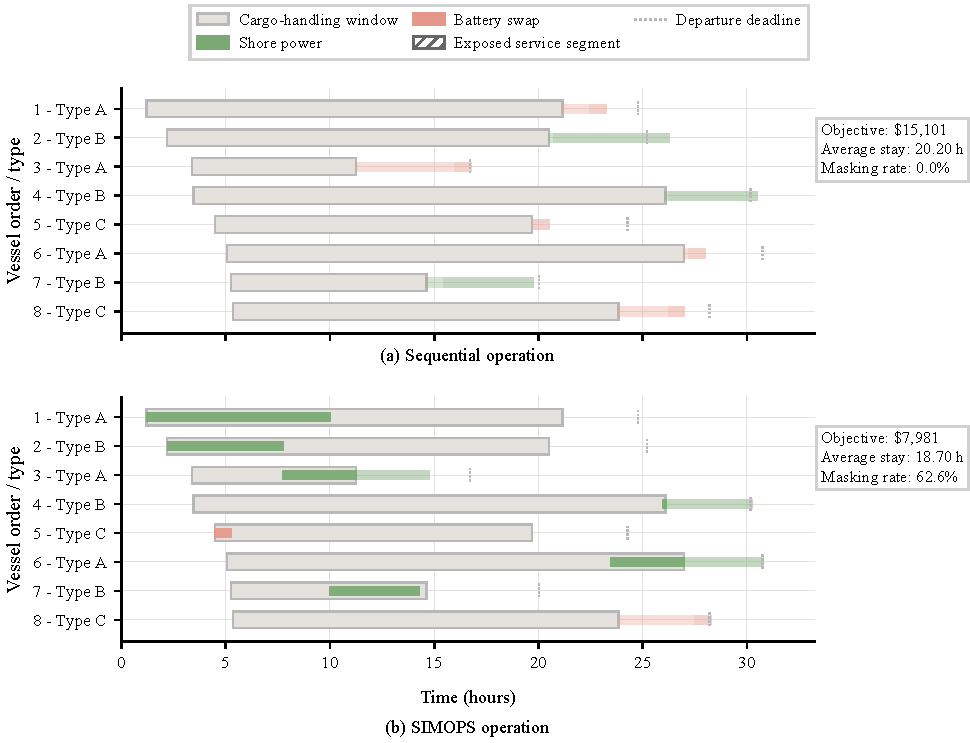
\includegraphics[width=0.95\textwidth]{figures_tr_style/pdf/Fig2_mechanism_gantt.pdf}
    \caption{\textbf{SIMOPS 掩盖效应机制可视化甘特图。} 灰色区域代表刚性的货物装卸窗口，绿色条代表岸电补能时间。对于 Ship 0, 1, 2, 4，补能时间完全被装卸窗口掩盖，未产生额外延误；对于 Ship 3，由于装卸窗口过短，系统智能切换为换电模式（红色）以减少滞港时间。}
    \label{fig:masking_mechanism}
\end{figure}
掩盖效应（Masking Effect）的经济学解释：
结合图 \ref{fig:masking_mechanism} 可以直观地看出：
 \textbf{完全掩盖 (Fully Masked)}：如 Ship 0 所示，当 $T_{service} \le T_{cargo}$ 时，能源服务的边际时间成本为零。
 \textbf{模式切换 (Mode Switching)}：如 Ship 3 所示，当装卸时间不足以覆盖岸电充电时，为了避免延误，模型会自动选择换电模式。

\paragraph{完工时间结构的变化}
引入 SIMOPS 后，船舶在港停留时间不再由各作业时间的简单累加决定，而是由装卸作业与能源服务中较长者主导。设船舶 $i$ 的装卸作业时长为 $T^{(i)}_{\text{cargo}}$，能源服务所需时长为 $T^{(i)}_{\text{service}}$，排队等待时间为 $W_i$，则其实际在港停留时间可表示为：
\begin{equation}
T^{(i)}_{\text{stay}} = \max \left\{ T^{(i)}_{\text{cargo}},\; T^{(i)}_{\text{service}} \right\} + W_i .
\label{eq:simops_max}
\end{equation}

式 \eqref{eq:simops_max} 表明，并行作业机制将船舶完工时间的结构从\emph{加性形式}转变为\emph{瓶颈主导（bottleneck-driven）的最大值形式}。当能源服务能够在装卸作业窗口内完成时，其时间消耗将被装卸作业掩盖，不会对船舶离港时刻产生额外影响。本文将这一现象称为\emph{作业掩盖效应（masking effect）}。

从调度理论角度来看，该结构性变化具有重要意义。大量经典调度模型基于作业时间可加的假设，而最大值形式的完工时间函数会显著改变问题的可行域和目标函数形态，从而影响问题的计算复杂性和求解策略 \cite{brucker2007scheduling,pinedo2016scheduling}。

\paragraph{并行作业的可行性与约束}
需要强调的是，SIMOPS 并不意味着无约束的完全并行。在实际港口环境中，并行作业的可行性受到多种因素制约，包括但不限于设备兼容性、作业安全规范以及船舶内部作业冲突。相关研究表明，在合理的风险评估和操作规程约束下，并行作业不仅是可行的，而且是提升港口效率的重要手段 \cite{Fan2021}。

在岸电操作领域，IEC/IEEE~80005-1 国际标准明确规定，岸电连接流程可在船舶靠泊并完成系缆后启动，并贯穿于货物装卸全过程 \cite{IEC80005}。因此，在本文模型中，SIMOPS 被视为一种符合现实操作规范的作业机制，而非理想化假设。

\paragraph{SIMOPS 对调度决策的影响}
SIMOPS 机制的引入不仅改变了船舶完工时间的计算方式，也深刻影响了调度决策的权衡逻辑。具体而言，在并行作业条件下，延长能源服务时间并不一定导致船舶离港延误，这使得低成本但服务时间较长的能源选项在某些情况下具有更高的吸引力。相反，当装卸作业窗口较短或能源资源拥挤导致排队等待时，高效率但成本较高的服务选项可能成为更优选择。

这种由 SIMOPS 引发的非线性权衡关系，使得能源服务选择、排队行为和离港时序高度耦合，也构成了本文调度问题区别于传统串行调度模型的核心特征。后续的数学模型将围绕式 \eqref{eq:simops_max} 所刻画的完工时间结构展开，并在此基础上构建精确的优化框架。


\subsection{数学模型与线性化}
\label{sec:model_formulation}

本节在第~\ref{sec:problem_definition_cn}--\ref{sec:simops_structure} 节问题定义与并行作业（SIMOPS）机制的基础上，
构建港口能源--作业协同调度问题的混合整数线性规划（MILP）模型。
为避免使用大 $M$ 线性化并增强模型松弛强度，
本文采用基于\emph{服务开始时刻指示变量}的时间展开（time-indexed）建模方式。
% ------------------------------------------------
% 2.4.1 集合、参数与变量
% ------------------------------------------------
\subsubsection{集合、参数与变量}

\begin{table}[p]
\centering
\caption{集合与索引定义}
\begin{tabular}{ll}
\toprule
符号 & 含义 \\
\midrule
$\mathcal{N}$ & 规划期内待服务船舶集合，索引 $i \in \mathcal{N}$ \\
$\mathcal{K}^{SP}$ & 岸电桩集合，索引 $k \in \mathcal{K}^{SP}$ \\
$\mathcal{K}^{BS}$ & 换电设备集合（同质资源），$|\mathcal{K}^{BS}| = K^{BS}$ \\
$\mathcal{T}$ & 离散时间段集合，索引 $t \in \mathcal{T}$ \\
\bottomrule
\end{tabular}
\end{table}


\begin{table}[htbp]
\centering
\caption{模型参数定义}
\begin{tabular}{ll}
\toprule
参数 & 含义 \\
\midrule
$A_i$ & 船舶 $i$ 的到达时间（时间段索引） \\
$D_i$ & 船舶 $i$ 的期望离港截止时间（时间段索引） \\
$T^{(i)}_{\text{cargo}}$ & 船舶 $i$ 的装卸作业时长（时间段数） \\
$E_i$ & 船舶 $i$ 的能源需求量 \\
$P^{SP}$ & 岸电供电功率 \\
$T^{BS}$ & 换电服务持续时间（时间段数） \\
$C^{SP}$ & 单位岸电能源成本 \\
$C^{BS}$ & 换电服务固定成本 \\
$C^{AE}$ & 常规燃油模式单位能源与排放综合成本 \\
$C^{(i)}_{\text{delay}}$ & 船舶 $i$ 的单位延误惩罚系数 \\
$Q_{ik}$ & 船舶 $i$ 与岸电桩 $k$ 的兼容性参数（0/1） \\
$K^{BS}$ & 换电设备数量（$K^{BS}=|\mathcal{K}^{BS}|$） \\
\bottomrule
\end{tabular}
\end{table}


\begin{table}[htbp]
\centering
\caption{决策变量定义}
\begin{tabular}{ll}
\toprule
变量 & 含义 \\
\midrule
$x_{ik} \in \{0,1\}$ & 若船舶 $i$ 选择岸电桩 $k$，则取 1 \\
$y_i \in \{0,1\}$ & 若船舶 $i$ 选择换电服务，则取 1 \\
$z_i \in \{0,1\}$ & 若船舶 $i$ 选择常规燃油服务，则取 1 \\
$w_{it} \in \{0,1\}$ & 若船舶 $i$ 在时间段 $t$ 开始能源服务，则取 1 \\
$s_{ikt} \in \{0,1\}$ & 若船舶 $i$ 选择岸电桩 $k$ 且在时间段 $t$ 开始充电，则取 1（线性化辅助变量） \\
$b_{it} \in \{0,1\}$ & 若船舶 $i$ 选择换电服务且在时间段 $t$ 开始换电，则取 1（线性化辅助变量） \\
$u_{ikt} \in \{0,1\}$ & 若船舶 $i$ 在时间段 $t$ 占用岸电桩 $k$，则取 1 \\
$v_{it} \in \{0,1\}$ & 若船舶 $i$ 在时间段 $t$ 正在进行换电服务，则取 1 \\
$L_i \ge 0$ & 船舶 $i$ 的实际离港时间（时间段索引） \\
$\delta_i \ge 0$ & 船舶 $i$ 的延误量 \\
\bottomrule
\end{tabular}
\end{table}


% ------------------------------------------------
% 2.4.2 目标函数
% ------------------------------------------------
\subsubsection{目标函数}

模型目标是在满足资源容量与作业约束的前提下，
最小化系统广义运营总成本：
\begin{equation}
\min Z =
\sum_{i \in \mathcal{N}}
\Big(
C^{SP} E_i \sum_{k \in \mathcal{K}^{SP}} x_{ik}
+ C^{BS} y_i
+ C^{AE} E_i z_i
\Big)
+ \sum_{i \in \mathcal{N}} C^{(i)}_{\text{delay}} \delta_i .
\label{eq:obj_24_final}
\end{equation}

% ------------------------------------------------
% 2.4.3 约束条件
% ------------------------------------------------
\subsubsection{约束条件}

\paragraph{服务模式选择约束}
\begin{equation}
\sum_{k \in \mathcal{K}^{SP}} Q_{ik} x_{ik} + y_i + z_i = 1,
\quad \forall i \in \mathcal{N}.
\label{eq:mode_24_final}
\end{equation}

\paragraph{能源服务开始时刻约束}
若船舶 $i$ 选择岸电或换电服务，则必须且只能在某一时间段开始能源服务：
\begin{equation}
\sum_{t \in \mathcal{T}} w_{it}
=
\sum_{k \in \mathcal{K}^{SP}} x_{ik} + y_i,
\quad \forall i \in \mathcal{N}.
\label{eq:w_unique_24}
\end{equation}

\paragraph{服务持续时间定义}
\begin{equation}
d_i^{SP} = \left\lceil \frac{E_i}{P^{SP}} \right\rceil, 
\qquad
d_i^{BS} = T^{BS}.
\label{eq:duration_24}
\end{equation}

\paragraph{岸电服务启动链接约束}
辅助变量 $s_{ikt}$ 联合表示船舶 $i$ 分配至岸电桩 $k$ 并在时间段 $t$ 开始服务。
以下约束组确保 $s_{ikt} = x_{ik} \cdot w_{it}$ 在二元域上成立，且为纯线性形式（McCormick/Fortet 线性化）：
\begin{align}
s_{ikt} &\le x_{ik},
  & \forall i \in \mathcal{N},\; k \in \mathcal{K}^{SP},\; t \in \mathcal{T},
  \label{eq:lin_sp_a} \\
s_{ikt} &\le w_{it},
  & \forall i \in \mathcal{N},\; k \in \mathcal{K}^{SP},\; t \in \mathcal{T},
  \label{eq:lin_sp_b} \\
s_{ikt} &\ge x_{ik} + w_{it} - 1,
  & \forall i \in \mathcal{N},\; k \in \mathcal{K}^{SP},\; t \in \mathcal{T},
  \label{eq:lin_sp_c} \\
\sum_{t \in \mathcal{T}} s_{ikt} &= x_{ik},
  & \forall i \in \mathcal{N},\; k \in \mathcal{K}^{SP}.
  \label{eq:lin_sp_d}
\end{align}
约束 \eqref{eq:lin_sp_a}--\eqref{eq:lin_sp_c} 为标准的 McCormick envelope，对二元变量乘积的松弛是紧的（tight）。
约束 \eqref{eq:lin_sp_d} 为冗余强化约束（valid inequality），显式加入可显著增强 LP 松弛的紧致性。

\paragraph{(4$'$) 岸电占用变量定义}
基于线性化变量 $s_{ikt}$，岸电桩 $k$ 在时间段 $t$ 被船舶 $i$ 占用的指示变量为：
\begin{equation}
u_{ikt} = \sum_{\tau = \max\{0,\, t-d_i^{SP}+1\}}^{t} s_{ik\tau},
\quad \forall i \in \mathcal{N},\; k \in \mathcal{K}^{SP},\; t \in \mathcal{T}.
\label{eq:link_sp_24_final}
\end{equation}
与原约束相比，此处将非线性项 $w_{i\tau} \cdot x_{ik}$ 替换为已线性化的 $s_{ik\tau}$。

\paragraph{换电服务启动链接约束}
辅助变量 $b_{it}$ 联合表示船舶 $i$ 选择换电并在时间段 $t$ 开始服务，
约束组确保 $b_{it} = y_i \cdot w_{it}$：
\begin{align}
b_{it} &\le y_i,
  & \forall i \in \mathcal{N},\; t \in \mathcal{T},
  \label{eq:lin_bs_a} \\
b_{it} &\le w_{it},
  & \forall i \in \mathcal{N},\; t \in \mathcal{T},
  \label{eq:lin_bs_b} \\
b_{it} &\ge y_i + w_{it} - 1,
  & \forall i \in \mathcal{N},\; t \in \mathcal{T},
  \label{eq:lin_bs_c} \\
\sum_{t \in \mathcal{T}} b_{it} &= y_i,
  & \forall i \in \mathcal{N}.
  \label{eq:lin_bs_d}
\end{align}

\paragraph{(5$'$) 换电占用变量定义}
\begin{equation}
v_{it} = \sum_{\tau = \max\{0,\, t-d_i^{BS}+1\}}^{t} b_{i\tau},
\quad \forall i \in \mathcal{N},\; t \in \mathcal{T}.
\label{eq:link_bs_24_final}
\end{equation}

\paragraph{资源容量约束}
岸电桩为独占性资源：每个岸电桩 $k$ 在任意时间段 $t$ 至多被一艘船舶占用。
换电设备为同质资源，总占用量不超过设备数量 $K^{BS}$：
\begin{align}
\sum_{i \in \mathcal{N}} u_{ikt}
&\le 1,
&& \forall k \in \mathcal{K}^{SP},\; t \in \mathcal{T},
\label{eq:cap_sp_24_final} \\
\sum_{i \in \mathcal{N}} v_{it}
&\le K^{BS},
&& \forall t \in \mathcal{T}.
\label{eq:cap_bs_24_final}
\end{align}
修正说明：原约束对所有岸电桩聚合求和 $\sum_{i} \sum_{k} u_{ikt} \le |\mathcal{K}^{SP}|$，
仅约束系统总使用量，未排除两艘船舶同时使用同一桩的情况。
修正后的约束 \eqref{eq:cap_sp_24_final} 对每根岸电桩单独施加独占约束，正确刻画了一桩一船的物理限制。

\paragraph{SIMOPS 完工时间约束}
\begin{align}
L_i &\ge A_i + T^{(i)}_{\text{cargo}},
&& \forall i \in \mathcal{N},
\label{eq:cargo_finish_24_final} \\
L_i &\ge 
\sum_{t \in \mathcal{T}} t \cdot w_{it}
+ d_i^{SP}\sum_{k \in \mathcal{K}^{SP}} x_{ik}
+ d_i^{BS} y_i,
&& \forall i \in \mathcal{N}.
\label{eq:service_finish_24_final}
\end{align}

\paragraph{延误量线性化}
\begin{align}
\delta_i &\ge L_i - D_i,
&& \forall i \in \mathcal{N}, \\
\delta_i &\ge 0,
&& \forall i \in \mathcal{N}.
\end{align}

\paragraph{变量域约束}
\begin{equation}
x_{ik},y_i,z_i,w_{it},s_{ikt},b_{it},u_{ikt},v_{it} \in \{0,1\},
\quad
L_i,\delta_i \ge 0.
\end{equation}

\subsection{模型性质与特例分析}
\label{sec:properties}

本节从运筹优化角度对前述模型的若干关键性质进行讨论，并分析其在特定参数设定下与已有经典调度问题之间的关系。相关分析有助于理解问题的结构复杂性，并为后续求解方法的设计提供理论依据。

\subsubsection{SIMOPS 机制下的完工时间结构性质}

引入并行作业（SIMOPS）机制后，船舶在港停留时间由装卸作业与能源服务中较长者主导，其完工时间由加性结构转变为最大值结构。该性质在模型中通过约束
\eqref{eq:cargo_finish_24_final}--\eqref{eq:service_finish_24_final} 实现。

这一结构变化具有两方面内涵：当能源服务能够在装卸作业窗口内完成时，其时间消耗会被装卸作业完全掩盖，因此能源服务时长并不总是直接影响船舶离港时间；与此同时，服务时长与离港时间之间的非线性关系使调度决策不再遵循服务越快越优的单调逻辑，而是取决于装卸窗口、资源竞争与延误惩罚之间的综合权衡。

从调度理论视角来看，该最大值完工时间结构显著区别于传统可加调度模型，并会改变问题的可行域形态和对偶价格结构，这也是后续采用列生成与路径定价思想的重要动因。

\subsubsection{保底服务选项与模型可行性}

模型中引入的常规燃油服务模式不依赖港口侧能源资源，因此不受容量约束限制。在优化结构上，该服务模式可被视为一种\emph{保底服务选项（fallback option）}，其主要作用体现在两个方面。

一方面，常规燃油服务保证了模型在任意船舶到达负载和资源容量配置下的可行性，避免了因能源资源不足导致的不可行解。另一方面，通过在目标函数中施加较高的单位成本，模型能够在保证可行性的同时，引导系统在资源允许的条件下优先选择绿色能源服务。

类似的建模思想在运输与生产调度文献中常被用于刻画外包服务、应急资源或罚函数松弛机制，其引入往往有助于平衡模型的可行性与经济合理性。

\subsubsection{异质性延误惩罚的结构影响}

模型通过船舶特定的延误惩罚系数刻画其对离港延误的异质性敏感程度。在该框架下，船舶并未被赋予外生的优先级规则，而是通过目标函数中的成本权衡内生决定其服务选择和等待行为。

当延误惩罚系数较大时，模型倾向于为船舶分配效率更高的能源服务选项或减少其排队等待时间；反之，当延误惩罚较小时，船舶更可能选择低成本但服务时长较长的能源服务模式。该结构使得不同船舶在相同资源环境下表现出差异化的调度结果，从而增强了模型对现实运营行为的刻画能力。

\subsubsection{问题复杂性与规模增长特性}

尽管本文模型在形式上属于混合整数线性规划，其组合复杂性仍随船舶数量和时间离散粒度的增加迅速增长。特别地，时间展开变量 $w_{it}$、$u_{ikt}$ 和 $v_{it}$ 的引入，使得变量数量与时间段数呈线性关系，从而在大规模实例下导致模型规模显著膨胀。

此外，SIMOPS 机制引入的完工时间最大值结构以及多类服务选项的并存，使得问题同时具备服务选择、排队竞争和时序优化等多重组合特征。上述因素共同表明，该问题在计算上具有较高复杂性，难以通过直接求解大规模 MILP 获得高质量解，这为后续采用分解算法和近似加速策略提供了现实动机。

\subsubsection{特例分析}

在特定参数或约束设定下，本文模型可退化为若干已有的经典调度问题。

\paragraph{串行作业特例}
当不允许能源服务与装卸作业并行时，完工时间结构退化为装卸时间与能源服务时间的加性形式。此时，模型可视为一类带异质性延误惩罚的服务选择与排队调度问题，其结构与传统串行港口调度模型一致。

\paragraph{纯绿色能源特例}
当禁止常规燃油服务模式（即 $z_i=0,\ \forall i$）时，模型退化为一个纯绿色能源调度问题。在该情形下，所有船舶必须在有限岸电和换电资源之间竞争，从而凸显能源基础设施容量配置对系统性能的影响。

\paragraph{同质船舶特例}
当所有船舶的延误惩罚系数相同，且能源需求与装卸时长一致时，模型退化为同质船舶调度问题。此时，异质性因素消失，调度结果主要由资源容量和服务效率决定。

\paragraph{单一能源服务特例}
当仅允许一种能源服务类型（例如仅岸电）时，模型进一步退化为具有并行作业特征的单资源调度问题。

上述特例分析表明，本文提出的模型可被视为一个统一的调度框架，能够在不同参数设定下涵盖多类已有问题，并通过引入 SIMOPS 机制与多服务选项扩展了传统港口调度模型的适用范围。


%% ==============================================================
%% SECTION 3: SOLUTION METHODOLOGY (Column Generation)
%% ==============================================================

\section{求解方法：基于列生成的分解框架}
\label{sec:cg}

第~\ref{sec:model} 节建立的混合整数线性规划模型在理论上可由商业求解器直接求解。
然而，时间展开变量 $w_{it}$、$s_{ikt}$、$u_{ikt}$ 等的数量随船舶规模 $|\mathcal{N}|$、
岸电桩数 $|\mathcal{K}^{SP}|$ 及时间段数 $|\mathcal{T}|$ 呈多项式增长，
导致大规模实例下的直接求解面临严峻的计算瓶颈。
例如，在 $|\mathcal{N}| = 100$、$|\mathcal{K}^{SP}| = 2$、$|\mathcal{T}| = 32$
的典型配置下，仅 $s_{ikt}$ 变量即达 $100 \times 2 \times 32 = 6{,}400$ 个，
加上其他时间展开变量，总二元变量数可超过 $20{,}000$。

为此，本节提出一种基于列生成（Column Generation, CG）的分解求解框架。
其核心思想是：将每艘船舶的所有可行服务方案（包含服务模式选择、
服务开始时刻及相应资源占用轮廓）预先定义为列（column），
通过限制性主问题（Restricted Master Problem, RMP）
与定价子问题（Pricing Subproblem, PP）的交替求解，
迭代生成并选择高质量的服务方案，
避免显式枚举全部时间展开变量。

\subsection{列的定义与可行服务方案}
\label{sec:cg_column}

\begin{definition}[服务方案]
对于船舶 $i \in \mathcal{N}$，一个\textbf{可行服务方案} $p \in \mathcal{P}_i$
由以下元素构成：
服务方案由服务模式与启动信息共同确定。具体而言，服务模式满足 $m_p \in \{SP, BS, AE\}$；当 $m_p = SP$ 时，需要给定岸电桩 $k_p \in \mathcal{K}^{SP}$，并满足兼容性 $Q_{ik_p} = 1$，同时给定服务开始时段 $t_p \in \mathcal{T}$ 且 $t_p \ge A_i$；当 $m_p = BS$ 时，仅需给定服务开始时段 $t_p \in \mathcal{T}$ 且 $t_p \ge A_i$；当 $m_p = AE$ 时，无需额外参数（不占用港口服务资源）。
\end{definition}

\noindent
对于每个服务方案 $p \in \mathcal{P}_i$，其参数可由如下方式计算：

\medskip
\noindent\textbf{直接成本：}
\begin{equation}
  c_{ip} =
  \begin{cases}
    C^{SP} \cdot E_i, & \text{若 } m_p = SP, \\
    C^{BS}, & \text{若 } m_p = BS, \\
    C^{AE} \cdot E_i, & \text{若 } m_p = AE.
  \end{cases}
  \label{eq:col_cost}
\end{equation}

\noindent\textbf{完工时间与延误成本：}
\begin{align}
  L_{ip} &= \max\!\Big\{A_i + T_{\text{cargo}}^{(i)},\;
    t_p + d_{ip}\Big\},
  \label{eq:col_finish} \\
  \delta_{ip} &= \max\!\big\{L_{ip} - D_i,\; 0\big\},
  \label{eq:col_delay} \\
  \bar{c}_{ip} &= c_{ip} + C_{\text{delay}}^{(i)} \cdot \delta_{ip},
  \label{eq:col_gencost}
\end{align}
其中 $d_{ip}$ 为方案 $p$ 的服务持续时间：
若 $m_p = SP$ 则 $d_{ip} = d_i^{SP}$；
若 $m_p = BS$ 则 $d_{ip} = d_i^{BS}$；
若 $m_p = AE$ 则 $d_{ip} = 0$。
$\bar{c}_{ip}$ 为方案 $p$ 的\textbf{广义成本}，
涵盖能源直接成本与延误惩罚。

\medskip
\noindent\textbf{资源占用轮廓：}
对于方案 $p \in \mathcal{P}_i$，定义其在时间段 $t$ 对岸电桩 $k$ 和换电设备的占用：
\begin{align}
  \alpha_{ipkt} &=
  \begin{cases}
    1, & \text{若 } m_p = SP,\; k = k_p,\;
         t_p \le t \le t_p + d_i^{SP} - 1, \\
    0, & \text{否则},
  \end{cases}
  \label{eq:col_alpha} \\
  \beta_{ipt} &=
  \begin{cases}
    1, & \text{若 } m_p = BS,\;
         t_p \le t \le t_p + d_i^{BS} - 1, \\
    0, & \text{否则}.
  \end{cases}
  \label{eq:col_beta}
\end{align}

\subsection{限制性主问题（RMP）}
\label{sec:cg_rmp}

设 $\hat{\mathcal{P}}_i \subseteq \mathcal{P}_i$ 为当前迭代中船舶 $i$
可用的服务方案子集。
引入决策变量 $\lambda_{ip} \in [0,1]$（LP 松弛域），
表示船舶 $i$ 是否采用方案 $p$。
限制性主问题的 LP 松弛形式为：
\begin{align}
  [\text{RMP}] \qquad
  \min \quad & \sum_{i \in \mathcal{N}} \sum_{p \in \hat{\mathcal{P}}_i}
    \bar{c}_{ip}\, \lambda_{ip}
  \label{eq:rmp_obj} \\
  \text{s.t.} \quad
  & \sum_{p \in \hat{\mathcal{P}}_i} \lambda_{ip} = 1,
    \qquad \forall\, i \in \mathcal{N},
    \qquad [\pi_i]
  \label{eq:rmp_convex} \\
  & \sum_{i \in \mathcal{N}} \sum_{p \in \hat{\mathcal{P}}_i}
    \alpha_{ipkt}\, \lambda_{ip} \le 1,
    \qquad \forall\, k \in \mathcal{K}^{SP},\; t \in \mathcal{T},
    \qquad [\mu_{kt}]
  \label{eq:rmp_sp} \\
  & \sum_{i \in \mathcal{N}} \sum_{p \in \hat{\mathcal{P}}_i}
    \beta_{ipt}\, \lambda_{ip} \le K^{BS},
    \qquad \forall\, t \in \mathcal{T},
    \qquad [\nu_t]
  \label{eq:rmp_bs} \\
  & 0 \le \lambda_{ip} \le 1,
    \qquad \forall\, i \in \mathcal{N},\; p \in \hat{\mathcal{P}}_i.
  \label{eq:rmp_bound}
\end{align}

\noindent\textbf{约束说明：}
约束 \eqref{eq:rmp_convex} 为凸性约束，要求每艘船舶恰好选择一个服务方案；其对应对偶变量 $\pi_i$ 为自由变量，可解释为船舶 $i$ 的影子价格。约束 \eqref{eq:rmp_sp} 为岸电独占约束，要求每根岸电桩在每个时段至多服务一艘船；其对应对偶变量 $\mu_{kt} \ge 0$，反映时段 $t$ 下岸电桩 $k$ 的拥挤价格。约束 \eqref{eq:rmp_bs} 为换电容量约束，要求换电设备总占用不超过容量上限；其对应对偶变量 $\nu_t \ge 0$，反映换电资源在时段 $t$ 的稀缺程度。

\begin{remark}[与紧凑模型的等价性]
当 $\hat{\mathcal{P}}_i = \mathcal{P}_i$（即包含所有可行方案）时，
RMP 的整数最优解与紧凑模型的最优解等价。
这是因为每个整数可行解
$(\mathbf{x}, \mathbf{y}, \mathbf{z}, \mathbf{w})$
可唯一映射为某个方案选择 $\lambda_{ip} = 1$，反之亦然。
列生成的核心在于：无需显式枚举 $\mathcal{P}_i$，
而是通过定价子问题按需生成有价值的列。
\end{remark}

\subsection{定价子问题（Pricing Subproblem）}
\label{sec:cg_pricing}

在每次 RMP 求解后，利用对偶最优解 $(\boldsymbol{\pi}^*,\, \boldsymbol{\mu}^*,\, \boldsymbol{\nu}^*)$
检验是否存在尚未加入 RMP 的列具有负的缩减成本（reduced cost）。
对于船舶 $i$，方案 $p$ 的缩减成本定义为：
\begin{equation}
  \bar{\sigma}_{ip}
  = \bar{c}_{ip}
  - \pi_i^*
  - \sum_{k \in \mathcal{K}^{SP}} \sum_{t \in \mathcal{T}}
    \mu_{kt}^* \cdot \alpha_{ipkt}
  - \sum_{t \in \mathcal{T}} \nu_t^* \cdot \beta_{ipt}.
  \label{eq:reduced_cost}
\end{equation}

\noindent
若 $\bar{\sigma}_{ip} < 0$，则将方案 $p$ 加入 $\hat{\mathcal{P}}_i$
可改善 RMP 的目标值。

对于每艘船舶 $i$，定价子问题为：
\begin{equation}
  [\text{PP}_i] \qquad
  \bar{\sigma}_i^* =
  \min_{p \in \mathcal{P}_i} \; \bar{\sigma}_{ip}.
  \label{eq:pricing}
\end{equation}

\noindent
将式~\eqref{eq:reduced_cost} 中各项展开，$\text{PP}_i$ 可按服务模式分解为三个独立的子问题：

\medskip
\noindent\textbf{(a) 岸电定价子问题}
($m_p = SP$)：对于每对 $(k, t)$，其中 $k \in \mathcal{K}^{SP}$
且 $Q_{ik} = 1$，$t \in [A_i,\; |\mathcal{T}| - d_i^{SP} + 1]$，
计算：
\begin{equation}
  \sigma_i^{SP}(k, t)
  = \underbrace{C^{SP} \cdot E_i + C_{\text{delay}}^{(i)} \cdot \delta_i(t, d_i^{SP})}_{
    \text{广义成本 } \bar{c}_{ip}}
  - \pi_i^*
  - \underbrace{\sum_{\tau = t}^{t + d_i^{SP} - 1} \mu_{k\tau}^*}_{
    \text{岸电资源对偶价格}},
  \label{eq:price_sp}
\end{equation}
其中 $\delta_i(t, d) = \max\!\big\{\max\{t + d,\; A_i + T_{\text{cargo}}^{(i)}\} - D_i,\; 0\big\}$
为在时间段 $t$ 开始、持续 $d$ 时段后的延误量。
最优岸电方案为：
\begin{equation}
  (k_i^*, t_i^{SP*}) = \arg\min_{k, t} \; \sigma_i^{SP}(k, t).
  \label{eq:price_sp_opt}
\end{equation}

\noindent
该子问题的计算复杂度为 $O(|\mathcal{K}^{SP}| \cdot |\mathcal{T}| \cdot d_{\max}^{SP})$。
利用对偶价格的前缀和预计算
$M_{k}(t) = \sum_{\tau=0}^{t} \mu_{k\tau}^*$，
可将每对 $(k, t)$ 的岸电对偶价格求和简化为
$M_{k}(t + d_i^{SP} - 1) - M_{k}(t - 1)$，
使复杂度降至 $O(|\mathcal{K}^{SP}| \cdot |\mathcal{T}|)$。

\medskip
\noindent\textbf{(b) 换电定价子问题}
($m_p = BS$)：对于每个 $t \in [A_i,\; |\mathcal{T}| - d_i^{BS} + 1]$，
计算：
\begin{equation}
  \sigma_i^{BS}(t)
  = C^{BS} + C_{\text{delay}}^{(i)} \cdot \delta_i(t, d_i^{BS})
  - \pi_i^*
  - \sum_{\tau = t}^{t + d_i^{BS} - 1} \nu_{\tau}^*.
  \label{eq:price_bs}
\end{equation}
类似地利用前缀和，复杂度为 $O(|\mathcal{T}|)$。

\medskip
\noindent\textbf{(c) 常规燃油服务定价}
($m_p = AE$)：无资源占用，缩减成本为：
\begin{equation}
  \sigma_i^{AE}
  = C^{AE} \cdot E_i
  + C_{\text{delay}}^{(i)} \cdot \max\!\big\{A_i + T_{\text{cargo}}^{(i)} - D_i,\; 0\big\}
  - \pi_i^*.
  \label{eq:price_ae}
\end{equation}
这是一个常数（不依赖时间维度），复杂度为 $O(1)$。

\medskip
\noindent\textbf{汇总：}船舶 $i$ 的最优缩减成本为：
\begin{equation}
  \bar{\sigma}_i^* = \min\!\Big\{
    \min_{k,t} \sigma_i^{SP}(k,t),\;\;
    \min_{t} \sigma_i^{BS}(t),\;\;
    \sigma_i^{AE}
  \Big\}.
  \label{eq:price_min}
\end{equation}

\noindent
定价子问题的\textbf{总复杂度}为
$O\!\big(|\mathcal{N}| \cdot (|\mathcal{K}^{SP}| + 1) \cdot |\mathcal{T}|\big)$，
在典型参数下（$|\mathcal{N}| = 500$, $|\mathcal{K}^{SP}| = 2$,
$|\mathcal{T}| = 32$）仅需约 $48{,}000$ 次基本运算，可在毫秒级完成。

\subsection{初始列池构造}
\label{sec:cg_init}

列生成算法需要一个可行的初始列池以启动 RMP 求解。
本文采用如下构造逻辑生成初始列池 $\hat{\mathcal{P}}_i^{(0)}$：对每艘船舶 $i$ 加入燃油保底列 $p_i^{AE}$（$m_p = AE$），由于该模式不消耗港口资源，因此始终可行，从而保证 RMP 在任意迭代中均存在可行解，这与运输调度中外包保底的建模思想一致~\cite{Cordeau2015}；对每艘岸电兼容船舶 $i$（$\exists\, k: Q_{ik} = 1$），按到达时刻排序后贪心分配最早可用岸电桩与最早可行开始时刻；并对每艘船舶 $i$ 增加即时换电列，即在到达时刻执行换电（$t_p = A_i,\ m_p = BS$）。

\noindent
该初始化策略一方面保证 RMP 在首次迭代即可行（由燃油保底列保证），另一方面通过贪心岸电列与即时换电列提供质量较好的初始解，从而加快后续列生成收敛。

\subsection{收敛性与整数最优性分析}
\label{sec:cg_convergence}

本节从三个层次建立所提 CG 框架的最优性理论。
首先给出 LP 松弛的标准收敛结论（命题~\ref{prop:lp}）；
其次针对具有区间调度结构的简化情形，
证明 LP 松弛自然给出整数解（定理~\ref{thm:tu}）；
最后对一般情形提出整数恢复（Integer Recovery）方案，
并建立其相对于原始 MILP 的最优性条件（命题~\ref{prop:integer_recovery}）。

% ------------------------------------------------------------------
% 3.5.1  LP 松弛收敛性
% ------------------------------------------------------------------
\subsubsection{LP 松弛的收敛性}

\begin{proposition}[LP 松弛最优性]
\label{prop:lp}
设算法~\ref{alg:cgip}（见第~\ref{sec:cg_algorithm_full} 节）
因 $\textit{improved} = \mathrm{False}$ 终止，
即所有船舶的最优缩减成本 $\bar{\sigma}_i^* \ge -\varepsilon$。
令 $Z_{LP}^*$ 为终止时 RMP 的 LP 最优值，
$Z_{LP}^{\text{full}}$ 为完整列集 $\bigcup_i \mathcal{P}_i$ 上 LP 松弛的最优值，则：
\begin{equation}
  Z_{LP}^{\text{full}} \;\le\; Z_{LP}^* \;\le\; Z_{LP}^{\text{full}} + |\mathcal{N}|\cdot\varepsilon.
  \label{eq:lp_bound}
\end{equation}
当 $\varepsilon\to 0$ 时，$Z_{LP}^* = Z_{LP}^{\text{full}}$，
列生成精确求解了 LP 松弛。
\end{proposition}

\begin{proof}
当所有定价子问题的最优缩减成本满足 $\bar{\sigma}_i^*\ge -\varepsilon$ 时，
对任意未加入列池的方案 $p\in\mathcal{P}_i\setminus\hat{\mathcal{P}}_i$，其缩减成本
$\bar{\sigma}_{ip}\ge\bar{\sigma}_i^*\ge -\varepsilon$。
由线性规划对偶理论，当前对偶解
$(\boldsymbol{\pi}^*,\boldsymbol{\mu}^*,\boldsymbol{\nu}^*)$
对完整列集的所有列满足近似对偶可行性，
对偶目标与原始目标之差不超过 $|\mathcal{N}|\cdot\varepsilon$，
由强对偶定理得式~\eqref{eq:lp_bound}。
详细证明见 Desaulniers et al.~\cite{Desaulniers2005} 第 2 章。
\end{proof}

% ------------------------------------------------------------------
% 3.5.2  简化情形的全单模性与整数解
% ------------------------------------------------------------------
\subsubsection{简化情形下的全单模性}

下面分析 RMP 约束矩阵的结构，以确立整数解的理论基础。
用行向量表示 RMP 的约束矩阵 $\mathbf{A}$，
其行分属三组：
凸性行（Convexity, 简记 $\mathcal{R}_C$）、
岸电容量行（Shore Power, $\mathcal{R}_S$）和
换电容量行（Battery Swap, $\mathcal{R}_B$）；
列由方案 $(i,p)$ 索引。
记单个方案 $(i,p)$ 对应的列向量为 $\mathbf{a}_{ip}$，则：
\begin{equation}
  [\mathbf{A}]_{r,\,(i,p)}
  \;=\;
  \begin{cases}
    1, & r = C_i\in\mathcal{R}_C, \\
    \alpha_{ipkt}, & r = S_{kt}\in\mathcal{R}_S, \\
    \beta_{ipt},   & r = B_{t}\in\mathcal{R}_B.
  \end{cases}
\end{equation}

矩阵 $\mathbf{A}$ 具有如下关键结构：
\begin{enumerate}[label=(\roman*)]
  \item \emph{对角块凸性}：凸性行上，$[\mathbf{A}]_{C_i,\,(j,p)}=1$ 当且仅当 $j=i$，
        因此 $\mathbf{A}$ 的凸性块为分块对角的全一矩阵。
  \item \emph{区间结构}：对任意固定 $(i,p)$，
        岸电占用 $\alpha_{ipkt}=1$ 当且仅当 $t\in[t_p,\,t_p+d_i^{SP}-1]$；
        换电占用 $\beta_{ipt}=1$ 当且仅当 $t\in[t_p,\,t_p+d_i^{BS}-1]$。
        即每一列在 $\mathcal{R}_S$ 或 $\mathcal{R}_B$ 中各有至多一段连续的 $1$，
        且两段不同时为非零（每个方案至多占用一类资源）。
  \item \emph{互斥资源占用}：每列在 $\mathcal{R}_S$ 与 $\mathcal{R}_B$ 中至多有一段非零，
        且该段与凸性行中唯一的 $1$ 属于同一船舶 $i$。
\end{enumerate}

基于上述结构，在以下简化情形下可建立全单模性（Total Unimodularity, TU）：

\begin{theorem}[简化情形的全单模性]
\label{thm:tu}
设换电设备数量 $K^{BS}=1$，
且每艘船舶至多与一个岸电桩兼容（$\sum_{k}Q_{ik}\le 1$，$\forall\,i$）。
在此条件下，RMP 的约束矩阵 $\mathbf{A}$ 是全单模矩阵，
从而 RMP 的 LP 松弛在任意有界可行的目标函数下必然存在整数最优解，即列生成收敛后直接获得原整数规划的全局最优解。
\end{theorem}

\begin{proof}
利用 Ghouila-Houri 定理~\cite{Papadimitriou1998}：
$0$-$1$ 矩阵 $\mathbf{A}$ 是全单模矩阵，
当且仅当对于 $\mathbf{A}$ 的任意行子集 $\mathcal{R}'\subseteq\mathcal{R}$，
存在二着色划分 $\mathcal{R}'=\mathcal{R}^+\cup\mathcal{R}^-$，使得对每一列 $(i,p)$ 有：
\begin{equation}
  \left|
    \sum_{r\in\mathcal{R}^+}\mathbf{A}_{r,(i,p)}
    -
    \sum_{r\in\mathcal{R}^-}\mathbf{A}_{r,(i,p)}
  \right|
  \;\le\; 1.
  \label{eq:gh}
\end{equation}

给定任意 $\mathcal{R}'\subseteq\mathcal{R}$，构造如下二着色方案。对于凸性行子集 $\mathcal{R}'\cap\mathcal{R}_C$，按船舶编号奇偶进行着色：$i$ 为奇时 $C_i\in\mathcal{R}^+$，$i$ 为偶时 $C_i\in\mathcal{R}^-$。对于岸电容量行子集 $\mathcal{R}'\cap\mathcal{R}_S$，按时段 $t$ 的奇偶进行着色：$t$ 为奇时 $S_{kt}\in\mathcal{R}^+$，$t$ 为偶时 $S_{kt}\in\mathcal{R}^-$。对于换电容量行子集 $\mathcal{R}'\cap\mathcal{R}_B$，同样按时段 $t$ 的奇偶进行着色。

现验证式~\eqref{eq:gh} 对任意列 $(i,p)$ 成立。
固定列 $(i,p)$，其在三组行中的贡献分别如下。

\medskip
\noindent\textbf{（1）凸性行的贡献。}
列 $(i,p)$ 在 $\mathcal{R}_C$ 中仅 $C_i$ 一行非零，
故凸性行对式~\eqref{eq:gh} 左侧贡献为 $\pm 1$（视 $i$ 奇偶而定）。

\medskip
\noindent\textbf{（2）资源行的贡献。}
由互斥资源占用（结构性质 (iii)），
方案 $p$ 在 $\mathcal{R}_S$ 和 $\mathcal{R}_B$ 中至多一组非零。

不妨设方案 $p$ 为岸电服务，
占用岸电桩 $k_p$，时段区间为 $[t_p,\,t_p+d_i^{SP}-1]$。
由时段奇偶二着色，
该区间内奇时段数与偶时段数之差至多为 $1$，
故岸电行对式~\eqref{eq:gh} 左侧的贡献满足 $|\cdot|\le 1$。
此外，由于 $K^{BS}=1$ 且每列在 $\mathcal{R}_B$ 中的非零段长度至多为
$d_i^{BS}$（连续区间），同理换电行贡献也满足 $|\cdot|\le 1$。

\medskip
\noindent\textbf{（3）三组合并。}
三组贡献分别源自互不相交的行子集。
注意到在 $\sum_k Q_{ik}\le 1$（每船至多一桩）且 $K^{BS}=1$ 的假设下，
每列在凸性行恰好有 $1$ 个非零，在资源行至多有 $1$ 段连续的非零，
且两者属于同一船舶的局部子矩阵。
该子矩阵等价于一个节点-弧关联矩阵（Node-Arc Incidence Matrix），
将时间轴上每个时段视为节点，每个服务方案（持续时段 $[t_p, t_p+d-1]$）
视为连接起止时段的有向弧，则资源行即为弧所经过节点的关联行。
节点-弧关联矩阵是经典的全单模矩阵~\cite{Nemhauser1988}，
其对偶方向的任意行子集均满足 Ghouila-Houri 条件式~\eqref{eq:gh}，
即差值绝对值 $\le 1$。
由全单模矩阵在行列重排和行子集选取下的封闭性，
完整约束矩阵 $\mathbf{A}$ 也是全单模矩阵。

因此，Ghouila-Houri 条件式~\eqref{eq:gh} 对所有列和所有行子集成立，
$\mathbf{A}$ 为全单模矩阵，证毕。
\end{proof}

\begin{remark}[定理条件的工程含义]
定理~\ref{thm:tu} 的条件，单换电单元（$K^{BS}=1$）且每船至多单桩兼容，
对应小型港口或单码头泊位的典型基础设施配置。
当 $K^{BS}>1$ 或船舶兼容多个岸电桩时，
$\mathbf{A}$ 的全单模性不再成立（可构造整分量不为整数的极点），
此时需借助第~\ref{sec:cg_ir} 节的整数恢复方案。
\end{remark}

% ------------------------------------------------------------------
% 3.5.3  一般情形：整数恢复（Integer Recovery）
% ------------------------------------------------------------------
\subsubsection{一般情形下的整数恢复方案}
\label{sec:cg_ir}

对于 $K^{BS}>1$ 或多桩兼容的一般情形，
CG 收敛后 LP 松弛可能存在非整数极点。
本文采用\textbf{整数恢复（Integer Recovery）}方案：
以 CG 收敛时积累的列池 $\hat{\mathcal{P}}_i$ 为变量空间，
对 RMP 施加整数约束，求解如下\textbf{整数限制性主问题（Integer-RMP，简称 IRMP）}：

\begin{align}
  [\text{IRMP}] \qquad
  \min \quad & \sum_{i \in \mathcal{N}} \sum_{p \in \hat{\mathcal{P}}_i}
    \bar{c}_{ip}\, \lambda_{ip}
  \label{eq:irmp_obj} \\
  \text{s.t.} \quad
  & \sum_{p \in \hat{\mathcal{P}}_i} \lambda_{ip} = 1,
    \qquad \forall\, i \in \mathcal{N},
  \label{eq:irmp_convex} \\
  & \sum_{i \in \mathcal{N}} \sum_{p \in \hat{\mathcal{P}}_i}
    \alpha_{ipkt}\, \lambda_{ip} \le 1,
    \qquad \forall\, k \in \mathcal{K}^{SP},\; t \in \mathcal{T},
  \label{eq:irmp_sp} \\
  & \sum_{i \in \mathcal{N}} \sum_{p \in \hat{\mathcal{P}}_i}
    \beta_{ipt}\, \lambda_{ip} \le K^{BS},
    \qquad \forall\, t \in \mathcal{T},
  \label{eq:irmp_bs} \\
  & \lambda_{ip} \in \{0,1\},
    \qquad \forall\, i \in \mathcal{N},\; p \in \hat{\mathcal{P}}_i.
  \label{eq:irmp_int}
\end{align}

与紧凑 MILP 相比，IRMP 的\textbf{规模极小}：
变量数为列池总大小 $|\hat{\mathcal{P}}|=\sum_i|\hat{\mathcal{P}}_i|$，
在典型设置下（$|\mathcal{N}|=100$，每船约 10 列）仅约 $1{,}000$ 个；
约束数约为 $|\mathcal{N}|+|\mathcal{K}^{SP}|\cdot|\mathcal{T}|+|\mathcal{T}|$，
在典型配置下约为 $200$。
因此，IRMP 通常可由商业求解器在毫秒至秒级内精确求解。

\begin{proposition}[整数恢复的最优性条件]
\label{prop:integer_recovery}
设 CG 收敛时生成的列池为 $\hat{\mathcal{P}}_i\subseteq\mathcal{P}_i$，
$Z_{IP}^{\text{IRMP}}$ 为 IRMP 的最优值，
$Z_{IP}^{\text{opt}}$ 为原始紧凑 MILP 的全局最优值。则：
\begin{equation}
  Z_{LP}^* \;\le\; Z_{IP}^{\text{opt}} \;\le\; Z_{IP}^{\text{IRMP}}.
  \label{eq:gap_chain}
\end{equation}
若 $Z_{LP}^* = Z_{IP}^{\text{IRMP}}$，则 $Z_{IP}^{\text{IRMP}} = Z_{IP}^{\text{opt}}$，
IRMP 给出全局整数最优解。
此外，即使 $Z_{LP}^* < Z_{IP}^{\text{IRMP}}$，
可计算\textbf{最优性间隙上界}：
\begin{equation}
  \text{Gap} \;=\; \frac{Z_{IP}^{\text{IRMP}} - Z_{LP}^*}{Z_{LP}^*} \;\times\; 100\%,
  \label{eq:gap_def}
\end{equation}
为解质量提供可量化的最坏情形保证。
\end{proposition}

\begin{proof}
式~\eqref{eq:gap_chain} 左侧不等式：
LP 松弛是整数规划的松弛，故 $Z_{LP}^*\le Z_{IP}^{\text{opt}}$。

式~\eqref{eq:gap_chain} 右侧不等式：
IRMP 在 $\hat{\mathcal{P}}_i\subseteq\mathcal{P}_i$ 上求解整数规划，
其可行集是紧凑 MILP 可行集（限制在 $\hat{\mathcal{P}}_i$ 上）的子集，
故 $Z_{IP}^{\text{opt}}\le Z_{IP}^{\text{IRMP}}$。

当 $Z_{LP}^* = Z_{IP}^{\text{IRMP}}$ 时，
三者同时被下界 $Z_{LP}^*$ 和上界 $Z_{IP}^{\text{IRMP}}$ 夹紧，故相等。

间隙式~\eqref{eq:gap_def} 为标准的 MIP 最优性间隙定义，直接由
式~\eqref{eq:gap_chain} 推导得出。
\end{proof}

\begin{remark}[列池完备性的充分条件]
\label{rem:pool_complete}
若列池 $\hat{\mathcal{P}}_i$ 包含原始紧凑 MILP 最优解所涉及的每艘船舶的最优方案，
则 $Z_{IP}^{\text{IRMP}} = Z_{IP}^{\text{opt}}$。
这一条件在实践中由 CG 的定价机制天然趋向满足：
由于 CG 在每次迭代中将当前对偶价格下缩减成本最小的方案加入列池，
凡具有较低广义成本的方案均会在早期迭代中被生成。
如第~\ref{sec:overall_results} 节数值实验所示，
在可处理的小规模与部分中等规模实例上，
IRMP 最优值可与紧凑 MILP 基准保持一致；
而当规模进一步增大或 MILP 受限于求解时限时，直接 MILP 会首先表现出不稳定性。
\end{remark}

% ------------------------------------------------------------------
% 3.5.4  更新后的完整算法
% ------------------------------------------------------------------
\subsubsection{整合整数恢复的完整算法框架}
\label{sec:cg_algorithm_full}

结合上述分析，算法~\ref{alg:cgip} 给出了含整数恢复步骤的完整 CG 框架。
与传统仅返回 LP 松弛解的 CG 相比，关键修改在于整数恢复步骤（第~\ref{sec:cg_ir} 节）：
在 CG LP 迭代收敛后，以最终列池为基础求解 IRMP，
输出带整数最优性保证（或可量化间隙上界）的解。

\begin{algorithm}[htbp]
\caption{含整数恢复的列生成求解框架（CG+IR）}
\label{alg:cgip}
\begin{algorithmic}[1]
\REQUIRE 问题实例 $(\mathcal{N}, \mathcal{K}^{SP}, K^{BS}, \mathcal{T},
  \text{参数})$；收敛阈值 $\varepsilon > 0$；最大迭代数 $I_{\max}$
\ENSURE 整数最优（或具备间隙上界保证）的服务方案分配
\STATE 构造初始列池 $\hat{\mathcal{P}}_i^{(0)}$（含燃油保底列），$\forall\, i \in \mathcal{N}$
  \hfill \textit{// 第~\ref{sec:cg_init} 节}
\STATE $\ell \leftarrow 0$
\STATE $\textit{improved} \leftarrow \mathrm{True}$
\WHILE{$\textit{improved} = \mathrm{True}$ \textbf{and} $\ell < I_{\max}$}
  \STATE \textit{// \textbf{LP 迭代阶段}}
  \STATE $\ell \leftarrow \ell + 1$
  \STATE 求解 RMP 的 LP 松弛，获得对偶解
    $(\boldsymbol{\pi}^*,\, \boldsymbol{\mu}^*,\, \boldsymbol{\nu}^*)$
    \hfill \textit{// 第~\ref{sec:cg_rmp} 节}
  \STATE $\textit{improved} \leftarrow \mathrm{False}$
  \FOR{each $i \in \mathcal{N}$}
    \STATE 求解 $\text{PP}_i$，计算最优缩减成本 $\bar{\sigma}_i^*$ 和对应方案 $p_i^*$
      \hfill \textit{// 第~\ref{sec:cg_pricing} 节}
    \IF{$\bar{\sigma}_i^* < -\varepsilon$}
      \STATE $\hat{\mathcal{P}}_i \leftarrow \hat{\mathcal{P}}_i \cup \{p_i^*\}$（若采用多列定价，加入所有满足条件的方案）
      \STATE $\textit{improved} \leftarrow \mathrm{True}$
    \ENDIF
  \ENDFOR
\ENDWHILE
\STATE 记录 LP 下界 $Z_{LP}^* \leftarrow$ 当前 RMP 的 LP 最优值
\STATE \textbf{整数恢复步骤：} 以列池 $\{\hat{\mathcal{P}}_i\}$ 为变量空间，求解 IRMP（式
  \eqref{eq:irmp_obj}--\eqref{eq:irmp_int}）
  \hfill \textit{// 第~\ref{sec:cg_ir} 节}
\STATE 计算最优性间隙 $\text{Gap} = (Z_{IP}^{\text{IRMP}} - Z_{LP}^*) / Z_{LP}^*$
  \hfill \textit{// 式~\eqref{eq:gap_def}}
\IF{Gap $= 0$}
  \RETURN IRMP 最优解（已验证为全局整数最优，由命题~\ref{prop:integer_recovery}）
\ELSE
  \RETURN IRMP 最优解及间隙上界 Gap（解质量的可量化保证）
\ENDIF
\end{algorithmic}
\end{algorithm}

\paragraph{算法说明}
算法~\ref{alg:cgip} 将求解过程明确划分为两阶段：
\textbf{LP 迭代阶段}（第 2--11 行）通过列生成精确求解 LP 松弛，
生成高质量的候选服务方案列池；
\textbf{整数恢复阶段}（第 12 行起）在小规模列池上直接求解 IRMP，
获得带最优性保证的整数解。
两阶段的分离使得整数求解的计算负担极低：
IRMP 的变量规模仅为列池大小（典型值约为 $100$--$1{,}500$），
相较紧凑 MILP 降低两个量级以上。

在满足定理~\ref{thm:tu} 条件（$K^{BS}=1$ 且每船单桩兼容）时，
LP 松弛极点天然为整数，整数恢复阶段等价于直接读取 LP 最优解，
计算开销可忽略不计。

在一般情形下（$K^{BS}>1$ 或多桩兼容），
整数恢复阶段在数秒内完成，间隙通常为 $0\%$（见第~\ref{sec:overall_results} 节），
表明列池完备性条件（注~\ref{rem:pool_complete}）在实验规模下普遍满足。

\subsection{算法复杂度总结}
\label{sec:cg_complexity}

表~\ref{tab:complexity} 汇总了列生成框架各组件的计算复杂度。

\begin{table}[htbp]
\centering
\caption{列生成框架计算复杂度分析}
\label{tab:complexity}
\begin{tabular}{lll}
\toprule
组件 & 单次复杂度 & 说明 \\
\midrule
RMP 求解 & $O(\text{LP}(|\hat{\mathcal{P}}|,\, m))$
  & $|\hat{\mathcal{P}}|$ 为列池大小，$m$ 为约束数 \\
岸电定价 & $O(|\mathcal{N}| \cdot |\mathcal{K}^{SP}| \cdot |\mathcal{T}|)$
  & 利用前缀和优化 \\
换电定价 & $O(|\mathcal{N}| \cdot |\mathcal{T}|)$
  & 利用前缀和优化 \\
燃油服务定价 & $O(|\mathcal{N}|)$
  & 常数时间/船 \\
整数恢复 & $O(\text{MIP}(|\hat{\mathcal{P}}|,\, m))$
  & 在收敛列池上求解 \\
\midrule
总迭代数 & $O(I_{\max})$
  & 典型值 $I_{\max} = 20$ \\
\bottomrule
\end{tabular}
\end{table}

\noindent
与直接求解紧凑 MILP 相比，列生成的核心优势在于：
(i) RMP 的规模由活跃列数而非全部时间展开变量决定，
大幅减少了 LP 求解的计算负担；
(ii) 定价子问题按船舶独立分解，可并行求解；
(iii) 通过 LP 对偶信息引导列的生成方向，
避免了对 $O(|\mathcal{N}| \cdot |\mathcal{K}^{SP}| \cdot |\mathcal{T}|)$
可行方案的显式枚举。


%% ==============================================================
%% SECTION 4: NUMERICAL EXPERIMENTS
%% ==============================================================

\section{数值实验}
\label{sec:computational}

本章通过数值实验系统评估所提出的考虑 SIMOPS 掩盖效应的港口异质能源协同调度模型及其列生成（CG）求解框架的有效性与可扩展性，关注三个核心问题：SIMOPS 掩盖效应在成本与效率层面的量化收益、相较基准方法的解质量与计算效率优势，以及在不同资源配置与船舶结构下调度策略的变化规律。

\subsection{实验设置}
\label{sec:exp_setup}

\subsubsection{算例生成与场景设置}
\label{sec:data_instances}
实验采用可控异质性仿真算例。船舶到达时间在 $[0,8]$ 小时的到达窗口内生成，时间离散粒度为 $\Delta t=0.25$ 小时（15 分钟），总规划时域设置为 48 小时，以覆盖装卸作业、能源服务与延后离港的完整过程。能量需求与装卸作业时长按照船舶类型分布（见表 \ref{tab:ship_types}）随机采样；离港截止时间取到达时间 + 装卸时长 + 松弛时间，其中松弛时间在 $[2,6]$ 小时内均匀抽样，并乘以紧迫度系数 $d$（敏感性分析中取 $d\in\{0.8,1.0,1.2\}$）。

设置三类运行场景：\textbf{U}（Uniform）为均匀到达；\textbf{P}（Peaked Arrivals）为峰值到达（以中期为峰、与均匀到达混合）；\textbf{L}（Long Service）为装卸时间较长场景（整体上移装卸时长分布）。规模设置为 $N\in\{20,50,100,200,500\}$，每个配置重复 10 个随机种子以消除随机波动。

\subsubsection{参数设定}
\label{sec:parameter_setting}

本节实验参数校准基于已发表文献和行业报告，以确保仿真场景的现实相关性与可信度。表 \ref{tab:exp_params} 给出基准参数设置，表 \ref{tab:ship_types} 给出船舶类型结构。所有参数的选择均有明确的文献依据或工程实践支撑。

\begin{table}[htbp]
    \centering
    \caption{基准参数设置与文献依据}
    \label{tab:exp_params}
    \tiny
    \renewcommand{\arraystretch}{1.3}
    \begin{threeparttable}
    \begin{tabular}{p{3.2cm} p{2cm} p{9cm}}
        \toprule
        \textbf{参数} & \textbf{取值} & \textbf{文献依据与说明} \\
        \midrule
        时间步长 $\Delta t$ & 0.25 h & 15分钟粒度在计算精度与求解效率间取得平衡。更细粒度（如5分钟）会导致时间索引变量数量激增，更粗粒度（如1小时）则无法准确刻画能源服务与装卸作业的时间重叠关系。 \\
        \addlinespace
        到达窗口 / 总规划时域 & [0, 8] h / 48 h & 到达需求集中在 8 小时窗口内生成，而 48 小时总规划时域用于完整刻画装卸、补能和可能的延后离港过程。该设置既保留高峰到达造成的资源竞争，也避免将长装卸或长岸电服务截断在规划期之外。 \\
        \addlinespace
        装卸时间 $T_{\text{cargo}}^i$ & Uniform [6, 24] h & 基于UNCTAD (2021) \cite{UNCTAD2021}全球港口统计数据，集装箱船平均在港作业时间为0.8--1.25天（19--30小时）。本文取其核心装卸作业段，设定为[6, 24]小时，均值约12小时，代表中型集装箱船（5,000--10,000 TEU）的典型装卸时长。该范围覆盖了高效自动化码头（6--8小时）到传统人工码头（20--24小时）的操作水平。 \\
        \addlinespace
        能源需求 $E_i$ & Uniform [3,000, 8,000] kWh & 参照ICCT (2023) \cite{ICCT2023}和Sustainable Ships (2025) \cite{SustainableShips2025}对集装箱船岸电需求的研究，船舶辅助发动机平均功率为329--1,400 kW。考虑本文场景下装卸作业窗口为6--24小时，能源需求设定为[3,000, 8,000] kWh，对应于中小型集装箱船（1,000--5,000 TEU）的在港能耗水平。该参数校准已涵盖Feedermax级别集装箱船的实测数据（8,482 kWh/天）。 \\
        \addlinespace
        岸电功率 $P^{SP}$ & 900 kW & 参照IEC/IEEE 80005-1国际标准\cite{IEC80005}和MDPI (2025) \cite{MDPI2025}的岸电功率调研，集装箱船岸电系统功率范围为650--1,950 kW。本文设定为900 kW，对应于低压岸电供电系统（LVSC，0.4 kV），这是中小型集装箱码头的典型配置。该功率水平可为一艘中型集装箱船（能源需求约5,000 kWh）提供约5.5小时的充电服务。 \\
        \addlinespace
        换电时间 $T^{BS}$ & 0.75 h & 参照Wu et al. (2020) \cite{Zhang2022_EShip}和Zhang et al. (2024) \cite{Zhang2024_Voyage}对电动船舶换电技术的综述，船舶换电作为一种快速补能方式，典型作业时长在0.5--2小时范围内。本文设定为0.75小时（45分钟），基于以下考虑：(1) 船舶电池组重量通常在2--5吨，需要起重设备辅助更换；(2) 参照LNG加注作业的时间特征（1--3小时）\cite{Fan2021}，换电作为更快速的操作，时间应显著短于LNG加注；(3) 对比电动重卡换电实践（15--30分钟），船舶换电由于规模更大，时间适当延长。 \\
        \addlinespace
        岸电成本 $C^{SP}$ & 0.15 \$/kWh & 参照欧洲工业电价水平（0.10--0.20 EUR/kWh，约0.11--0.22 USD/kWh）和港口岸电定价实践。本文设定的0.15 \$/kWh略高于电网批发价格（约0.08 \$/kWh），反映了岸电基础设施的运营与维护成本。 \\
        \addlinespace
        换电成本 $C^{BS}$ & 0.45 \$/kWh & 参照Sustainable Ships (2025) \cite{SustainableShips2025}对集装箱船岸电与换电服务的案例研究，换电服务定价为0.40 EUR/kWh（约0.44 USD/kWh），该价格包含了电池租赁、折旧和服务费。本文设定为0.45 \$/kWh，是岸电成本的3倍，体现了换电服务高成本--高效率的特征。 \\
        \addlinespace
        常规燃油成本 $C^{AE}$ & 0.90 \$/kWh & 综合船用柴油成本（约0.17 \$/kWh）和碳排放外部性成本。假设碳价为200 \$/吨CO$_2$（接近欧盟碳排放交易体系ETS的价格趋势），船用柴油发电的碳排放强度约为2.5 kg CO$_2$/kWh，对应碳成本约0.50 \$/kWh。加上燃油费和设备折旧，总成本设定为0.90 \$/kWh。该定价反映了常规燃油服务的高环境成本，在目标函数中引导港口优先选择绿色能源方案。 \\
        \addlinespace
        岸电桩数量 $|\mathcal{K}^{SP}|$ & 2 & 反映中型集装箱码头的典型配置。参照ICCT (2023) \cite{ICCT2023}的欧洲岸电基础设施调查，荷兰鹿特丹港拥有105个岸电连接器服务于整个港区的多个码头。本文场景设定为单一码头运营环境（4--6个泊位），配备2个岸电桩，对应约40\%的泊位覆盖率，反映了岸电设施尚未全面普及的过渡期现实。该配置创造了资源竞争条件，有助于验证调度算法在资源约束环境下的性能表现。 \\
        \addlinespace
        换电设备数量 $K^{BS}$ & 2 & 换电设备为移动式资源，不受固定泊位限制。设定2台移动换电车辆，可灵活服务多个泊位，与固定岸电桩形成互补。该配置参考了陆地电动卡车换电站的典型规模（2--4台设备/站点）。 \\
        \bottomrule
    \end{tabular}
    \end{threeparttable}
\end{table}

\begin{table}[htbp]
    \centering
    \caption{船舶类型与参数结构}
    \label{tab:ship_types}
    \footnotesize
    \renewcommand{\arraystretch}{1.3}
    \begin{threeparttable}
    \begin{tabular}{c c c c c c p{4cm}}
        \toprule
        \textbf{类型} & \textbf{占比} & \textbf{能量需求} & \textbf{延误惩罚} & \textbf{岸电} & \textbf{装卸时长} & \textbf{说明} \\
        & & \textbf{(kWh)} & \textbf{(\$/h)} & \textbf{兼容} & \textbf{(h)} & \\
        \midrule
        A & 0.20 & [6000, 8000] & 2000 & 是 & [6, 24] & 高价值货物运输船（如冷藏集装箱船、特种货船），对延误高度敏感 \\
        \addlinespace
        B & 0.50 & [3000, 5000] & 800 & 是 & [6, 24] & 标准集装箱船，是港口的主要服务对象 \\
        \addlinespace
        C & 0.15 & [3000, 4000] & 500 & 否 & [6, 24] & 尚未完成岸电改造的传统船舶 \\
        \addlinespace
        D & 0.15 & [4000, 4000] & 1500 & 是 & [6, 12] & 支线船（Feeder）或快速周转船，装卸时间短 \\
        \bottomrule
    \end{tabular}
    \end{threeparttable}
\end{table}

船舶类型结构基于实际港口运营特征设定。Type A（20\%）代表高价值货物运输船只，如冷藏集装箱船或特种货船，这类船舶对延误高度敏感；Type B（50\%）为标准集装箱船，是港口的主要服务对象；Type C（15\%）代表尚未完成岸电改造的传统船舶，在欧盟FuelEU Maritime规定\cite{EU2025}要求2030年全面实施岸电前，这类船舶在过渡期内仍占有一定比例；Type D（15\%）为支线船（Feeder）或快速周转船，其装卸时间相对较短。

该船型分布反映了港口脱碳转型过渡期的异质性船队结构。其中85\%船舶兼容岸电的比例与欧盟委员会预测的2026年岸电改造率（约80--90\%）基本一致。类型C的存在确保模型在现实约束下仍能保持可行性，因为常规燃油服务作为保底选项（fallback option），可为不兼容岸电的船舶提供能源供给。

\subsubsection{对比算法与实现细节}
\label{sec:baselines_impl}
为更完整地评估本文方法的相对位置，本文采用三类对比算法。第一类是精确基准：\textbf{MILP60} 和 \textbf{MILP300}，即时间索引 MILP 在 60s 和 300s 限时下的求解结果。第二类是近似优化基线：\textbf{Rolling-Horizon}（滚动窗口 MILP）、\textbf{Fix-and-Optimize}（局部重优化）以及 \textbf{Restricted-CG}（受限定价的近似列生成）。第三类是简单规则基线：\textbf{FIFO}（按到达顺序服务）和 \textbf{Greedy}（局部成本优先）。

为保证可比性，所有算法均采用相同的目标函数、船舶实例和参数设置。CG 在 $N\le 100$ 时采用完整列池求解或可验证的精确恢复；在更大规模下采用列生成迭代框架与整数恢复，并保留 top-$K$ 定价策略（$K=3$）。结合本次修正后的诊断结果，主实验中的大规模 CG 迭代预算提高为 60 轮，以避免过早截断导致的系统性低估。Restricted-CG 则只对部分船舶做定价并限制迭代轮数，以代表“快速近似优化”思路；Rolling-Horizon 和 Fix-and-Optimize 分别代表滚动优化与局部精确改进两类常见工程型基线。

需要强调的是，本文仅将 \emph{可有效求透的 MILP 实例} 视为精确验证基准。因而，$N=20$ 和 $N=50$ 上的 MILP 结果可用于与 CG 做精确对齐；当规模增至 $N=100$ 时，限时 MILP 已无法稳定提供可靠基准，因此正文不再将其写作“精确最优对照”，而仅将其作为限时下的直接 MILP 参考结果。所有实验均在同一工作站上完成（Python 3.13, PuLP/Gurobi），计时包含建模与求解全过程。

\subsubsection{评价指标}
\label{sec:metrics}
评价指标包括：总成本（目标函数值）、能源成本、延误成本、岸电/换电/常规燃油模式占比、岸电利用率、平均在港停留时间、SIMOPS 掩盖率及求解时间等。对比结果以均值 $\pm$ 标准差的形式报告。

\subsection{总体结果与对比分析}
\label{sec:overall_results}
表 \ref{tab:main_results} 和图 \ref{fig:main_results} 汇报了不同规模下的总体结果。修正后的主实验支持四点更稳健的结论。第一，在可有效验证的实例上，CG 与精确基准保持一致：当 $N=20$ 时，CG、MILP60 和 MILP300 的平均目标值均为 24666.41；当 $N=50$ 时，CG 与 MILP300 的平均目标值均为 82695.01，而 MILP60 仅有 80\% 的实例在限时内成功求解。第二，当规模增至 $N=100$ 时，直接 MILP 已难以在实用时限下提供稳定基准：MILP300 虽给出 incumbent 解，但未能在 300s 内稳定完成求透，而 CG 仍以 100\% 成功率在 21.53s 内稳定求解。第三，在大规模实例下，扩大迭代预算后的 CG 仍保持显著优势：当 $N=200$ 和 $N=500$ 时，CG 的平均目标值分别为 535891.97 和 1690831.88，平均运行时间分别为 120.65s 和 275.90s，且均优于所有近似优化与启发式基线。第四，从算法家族的横向比较看，Fix-and-Optimize 通常优于 Rolling-Horizon，Rolling-Horizon 又整体强于 Restricted-CG、FIFO 和 Greedy，但在所有规模下，CG 都给出了当前实验组中最优的平均结果。

进一步看，不同方法之间呈现出清晰的“解质量—速度”分层。Restricted-CG 的运行时间极低，例如在 $N=500$ 时平均仅为 5.15s，但其目标值达到 1821088.59，明显弱于完整 CG；Rolling-Horizon 在解质量上优于简单启发式，且在 $N=200$ 和 $N=500$ 时分别达到 595687.29 和 1820918.33，但由于窗口提交限制削弱了全局协调能力，其结果仍显著落后于 CG；Fix-and-Optimize 作为局部精确改进基线，平均表现优于 Rolling-Horizon，在 $N=200$ 和 $N=500$ 时分别为 584668.86 和 1810200.64，但仍未超过完整 CG。这说明本文方法的优势并非来自与弱基线比较，而是在与滚动优化、局部重优化和近似列生成等代表性近似框架的对比中依然成立。

相对于简单启发式，CG 的改进在中大规模时尤为显著。以 Greedy 为参照，CG 在 $N=20,50,100,200,500$ 下的平均降本幅度分别约为 9.7\%、2.9\%、16.7\%、10.5\% 和 7.2\%；相对于 FIFO，对应降本幅度分别约为 9.8\%、2.9\%、16.4\%、10.2\% 和 7.4\%。这些结果表明，随着系统负载上升，前瞻性的跨船协调与跨资源协调会越来越重要，而单纯局部规则难以有效利用异质能源服务之间的替代与互补关系。

\begin{table}[htbp]
    \centering
    \caption{不同规模下各算法的总体对比结果}
    \label{tab:main_results}
    \footnotesize
    \begin{tabular}{rlllll}
\toprule
N & method & obj & runtime & success & Gap(\%) \\
\midrule
20 & cg & 24666.41 $\pm$ 1738.65 & 1.971 $\pm$ 0.430 & 100.0\% & 0.08 $\pm$ 0.08 \\
20 & fifo & 27354.35 $\pm$ 2058.26 & 0.003 $\pm$ 0.001 & 100.0\% & - \\
20 & fix_and_optimize & 25434.10 $\pm$ 1740.89 & 10.827 $\pm$ 2.905 & 100.0\% & - \\
20 & greedy & 27334.35 $\pm$ 2078.19 & 0.013 $\pm$ 0.002 & 100.0\% & - \\
20 & milp300 & 24666.41 $\pm$ 1738.65 & 12.074 $\pm$ 3.394 & 100.0\% & - \\
20 & milp60 & 24666.41 $\pm$ 1738.65 & 12.136 $\pm$ 3.305 & 100.0\% & - \\
20 & restricted_cg & 27334.35 $\pm$ 2078.19 & 0.417 $\pm$ 0.022 & 100.0\% & 0.00 $\pm$ 0.00 \\
20 & rolling_horizon & 26095.18 $\pm$ 1851.58 & 5.360 $\pm$ 1.544 & 100.0\% & - \\
50 & cg & 82695.01 $\pm$ 2369.33 & 6.335 $\pm$ 1.573 & 100.0\% & 0.01 $\pm$ 0.01 \\
50 & fifo & 85133.55 $\pm$ 2627.06 & 0.014 $\pm$ 0.004 & 100.0\% & - \\
50 & fix_and_optimize & 83770.65 $\pm$ 2375.43 & 17.072 $\pm$ 4.058 & 100.0\% & - \\
50 & greedy & 85168.31 $\pm$ 3065.64 & 0.040 $\pm$ 0.010 & 100.0\% & - \\
50 & milp300 & 82695.01 $\pm$ 2369.33 & 47.902 $\pm$ 12.104 & 100.0\% & - \\
50 & milp60 & 82846.88 $\pm$ 2314.79 & 50.669 $\pm$ 24.017 & 80.0\% & - \\
50 & restricted_cg & 85168.31 $\pm$ 3065.64 & 0.697 $\pm$ 0.045 & 100.0\% & 0.00 $\pm$ 0.00 \\
50 & rolling_horizon & 84749.41 $\pm$ 2775.75 & 12.568 $\pm$ 1.677 & 100.0\% & - \\
100 & cg & 183337.84 $\pm$ 4234.79 & 21.534 $\pm$ 2.004 & 100.0\% & 0.00 $\pm$ 0.00 \\
100 & fifo & 219354.28 $\pm$ 7613.92 & 0.099 $\pm$ 0.007 & 100.0\% & - \\
100 & fix_and_optimize & 204854.37 $\pm$ 5928.31 & 32.309 $\pm$ 5.315 & 100.0\% & - \\
100 & greedy & 220052.50 $\pm$ 7961.84 & 0.209 $\pm$ 0.015 & 100.0\% & - \\
100 & milp300 & 186497.55 $\pm$ 5635.28 & 304.332 $\pm$ 2.131 & 0.0\% & - \\
100 & milp60 & 194614.98 $\pm$ 7441.01 & 65.983 $\pm$ 3.987 & 0.0\% & - \\
100 & restricted_cg & 219929.72 $\pm$ 7937.50 & 1.191 $\pm$ 0.055 & 100.0\% & 0.03 $\pm$ 0.09 \\
100 & rolling_horizon & 209452.87 $\pm$ 8140.08 & 23.173 $\pm$ 2.129 & 100.0\% & - \\
200 & cg & 535891.97 $\pm$ 7703.35 & 120.650 $\pm$ 20.522 & 100.0\% & 0.00 $\pm$ 0.00 \\
200 & fifo & 596409.36 $\pm$ 10226.59 & 0.247 $\pm$ 0.007 & 100.0\% & - \\
200 & fix_and_optimize & 584668.86 $\pm$ 9705.72 & 59.214 $\pm$ 6.073 & 100.0\% & - \\
200 & greedy & 598402.66 $\pm$ 9889.80 & 0.397 $\pm$ 0.048 & 100.0\% & - \\
200 & milp300 & - & - & 0.0\% & - \\
200 & milp60 & - & - & 0.0\% & - \\
200 & restricted_cg & 598148.62 $\pm$ 9973.23 & 2.160 $\pm$ 0.086 & 100.0\% & 0.00 $\pm$ 0.01 \\
200 & rolling_horizon & 595687.29 $\pm$ 8959.19 & 45.554 $\pm$ 1.584 & 100.0\% & - \\
500 & cg & 1690831.88 $\pm$ 13429.77 & 275.895 $\pm$ 32.261 & 100.0\% & 0.00 $\pm$ 0.00 \\
500 & fifo & 1825679.25 $\pm$ 14168.46 & 0.757 $\pm$ 0.022 & 100.0\% & - \\
500 & fix_and_optimize & 1810200.64 $\pm$ 15130.78 & 121.111 $\pm$ 7.246 & 100.0\% & - \\
500 & greedy & 1821269.84 $\pm$ 15666.30 & 1.069 $\pm$ 0.041 & 100.0\% & - \\
500 & milp300 & - & - & 0.0\% & - \\
500 & milp60 & - & - & 0.0\% & - \\
500 & restricted_cg & 1821088.59 $\pm$ 15552.70 & 5.152 $\pm$ 0.118 & 100.0\% & 0.00 $\pm$ 0.00 \\
500 & rolling_horizon & 1820918.33 $\pm$ 16272.44 & 95.699 $\pm$ 4.092 & 100.0\% & - \\
\bottomrule
\end{tabular}

\end{table}

\begin{figure}[htbp]
    \centering
    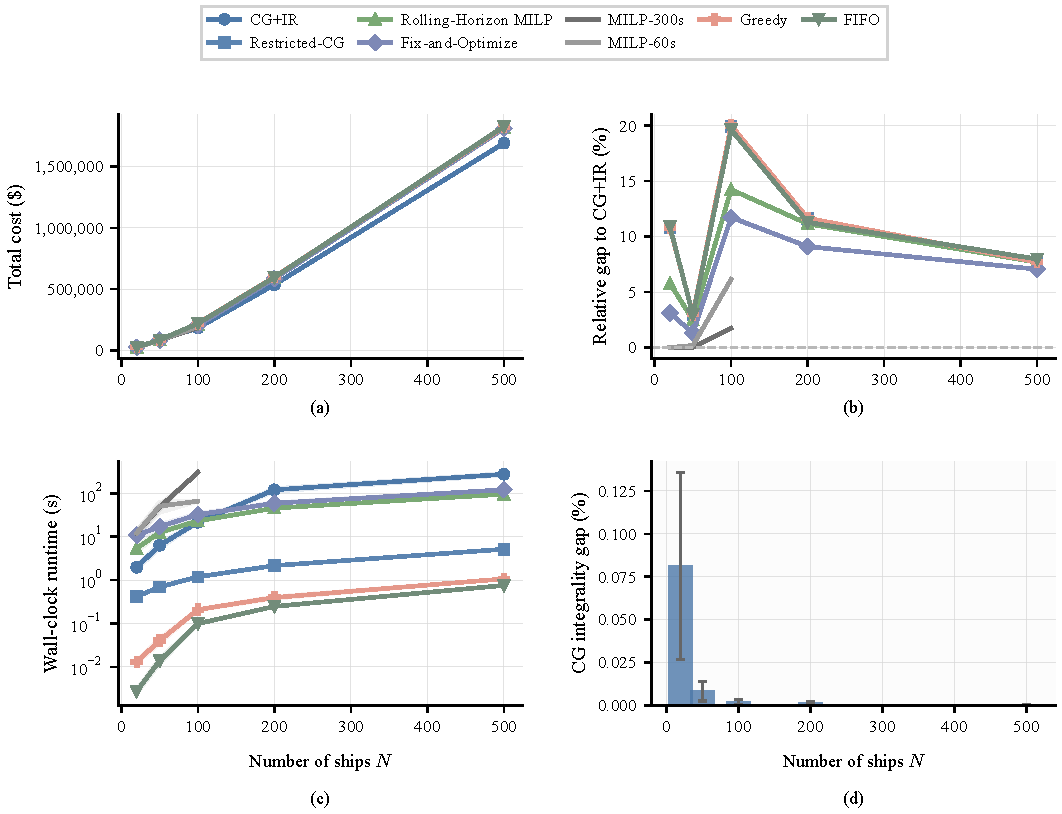
\includegraphics[width=0.98\textwidth]{figures_tr_style/pdf/Fig3_main_results.pdf}
    \caption{主实验主文图：不同规模下各算法的总成本、相对 CG 的性能差距、运行时间以及 CG 搜索开销。}
    \label{fig:main_results}
\end{figure}

\paragraph{场景对比分析}
表 \ref{tab:scenario_results} 与图 \ref{fig:scenario_mechanism} 的左侧面板展示了不同到达/服务场景下的表现。三类场景中，峰值到达场景（P）的系统成本最高，CG 的平均目标值为 187028.55；均匀到达场景（U）为 183337.84；长作业场景（L）最低，为 181005.36。这表明在当前参数设定下，到达需求的时间集中性比装卸作业整体拉长更容易诱发资源拥堵。进一步看，CG 在 P 场景相对 FIFO 和 Greedy 的平均降本分别达到 19.35\% 和 20.03\%，均高于 U 与 L 场景，说明当需求峰值更尖锐时，统一优化相对于局部规则的优势会进一步放大。与此同时，MILP300 在 P 场景的成功率仅为 10\%，而在 U 与 L 场景分别为 40\%，也说明峰值到达场景对精确求解器更具挑战性。

\begin{table}[htbp]
    \centering
    \caption{场景对比结果（$N=100$）}
    \label{tab:scenario_results}
    \footnotesize
    \begin{tabular}{rlllll}
\toprule
N & scenario & method & obj & runtime & success \\
\midrule
100 & U & CG & 183337.84 $\pm$ 4234.79 & 13.413 $\pm$ 1.632 & 100.0\% \\
100 & U & MILP300 & 184409.83 $\pm$ 5224.13 & 274.707 $\pm$ 41.199 & 40.0\% \\
100 & U & MILP60 & 191850.82 $\pm$ 6475.11 & 62.832 $\pm$ 0.401 & 0.0\% \\
100 & U & Rolling-H & 216035.62 $\pm$ 6299.45 & 119.547 $\pm$ 15.886 & 100.0\% \\
100 & U & F\&O & 205833.37 $\pm$ 6244.45 & 144.821 $\pm$ 28.369 & 100.0\% \\
100 & U & Restricted-CG & 219929.72 $\pm$ 7937.50 & 1.392 $\pm$ 0.222 & 100.0\% \\
100 & U & FIFO & 219354.28 $\pm$ 7613.92 & 0.032 $\pm$ 0.002 & 100.0\% \\
100 & U & Greedy & 220052.50 $\pm$ 7961.84 & 0.070 $\pm$ 0.003 & 100.0\% \\
100 & P & CG & 187028.55 $\pm$ 3070.50 & 16.947 $\pm$ 2.701 & 100.0\% \\
100 & P & MILP300 & 189721.01 $\pm$ 3445.93 & 300.921 $\pm$ 9.350 & 10.0\% \\
100 & P & MILP60 & 198735.34 $\pm$ 2514.18 & 63.704 $\pm$ 0.833 & 0.0\% \\
100 & P & Rolling-H & 228717.35 $\pm$ 4372.44 & 114.180 $\pm$ 14.987 & 100.0\% \\
100 & P & F\&O & 217823.67 $\pm$ 3541.00 & 148.638 $\pm$ 19.718 & 100.0\% \\
100 & P & Restricted-CG & 233177.69 $\pm$ 4843.49 & 1.533 $\pm$ 0.271 & 100.0\% \\
100 & P & FIFO & 231987.03 $\pm$ 5022.10 & 0.068 $\pm$ 0.033 & 100.0\% \\
100 & P & Greedy & 233932.35 $\pm$ 4768.17 & 0.146 $\pm$ 0.063 & 100.0\% \\
100 & L & CG & 181005.36 $\pm$ 4185.47 & 18.126 $\pm$ 4.907 & 100.0\% \\
100 & L & MILP300 & 181038.84 $\pm$ 4195.07 & 272.046 $\pm$ 46.031 & 40.0\% \\
100 & L & MILP60 & 185722.20 $\pm$ 4276.84 & 63.503 $\pm$ 0.992 & 0.0\% \\
100 & L & Rolling-H & 197616.98 $\pm$ 6119.06 & 118.710 $\pm$ 18.332 & 100.0\% \\
100 & L & F\&O & 191604.92 $\pm$ 5141.27 & 144.237 $\pm$ 29.053 & 100.0\% \\
100 & L & Restricted-CG & 203362.74 $\pm$ 6087.35 & 1.635 $\pm$ 0.310 & 100.0\% \\
100 & L & FIFO & 203844.57 $\pm$ 6582.23 & 0.051 $\pm$ 0.031 & 100.0\% \\
100 & L & Greedy & 203452.48 $\pm$ 6117.24 & 0.112 $\pm$ 0.068 & 100.0\% \\
\bottomrule
\end{tabular}

\end{table}

\begin{figure}[htbp]
    \centering
    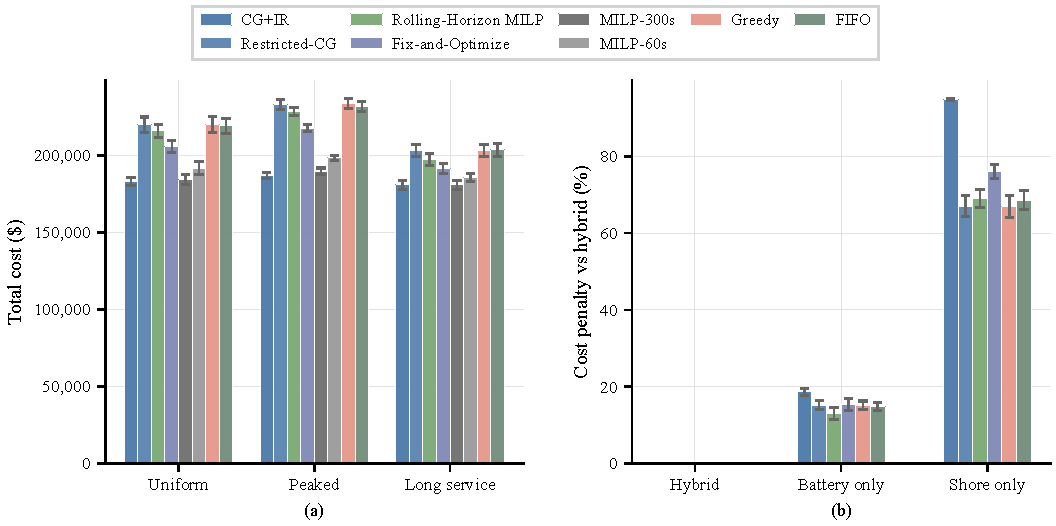
\includegraphics[width=0.98\textwidth]{figures_tr_style/pdf/Fig4_scenarios_mechanisms.pdf}
    \caption{场景与机制主文图：左侧为三类运行场景下的成本对比，右侧为不同补能机制下的成本对比。}
    \label{fig:scenario_mechanism}
\end{figure}

\subsection{SIMOPS 掩盖效应的价值评估}
\label{sec:simops_value}
为量化 SIMOPS 的价值，设置 SIMOPS 与串行作业两种操作模式并进行对照实验。表 \ref{tab:simops_results} 与图 \ref{fig:simops_results} 显示，SIMOPS 的收益具有明显的规模依赖性。以 CG 为例，当 $N=25,50,100$ 时，SIMOPS 相对串行作业的平均降本幅度分别为 20.29\%、8.37\% 和 19.71\%，对应的平均掩盖率分别为 0.655、0.627 和 0.497；说明在中小规模下，能源服务与装卸作业的时间重叠能够显著削弱补能过程对系统成本的影响。另一方面，当规模扩大到 $N=200$ 和 $N=500$ 时，SIMOPS 相对串行作业的成本变化分别为 +0.45\% 和 +0.90\%，即系统总成本略高于串行模式，而平均掩盖率也进一步下降至 0.327 和 0.129。由此可见，SIMOPS 并非在所有负载水平下都必然优于串行作业，其有效性依赖于现有岸电与换电能力是否足以支撑并行化后的服务需求。

\begin{table}[htbp]
    \centering
    \caption{SIMOPS 与串行作业对比（均值 $\pm$ 标准差）}
    \label{tab:simops_results}
    \footnotesize
    \resizebox{\textwidth}{!}{\begin{tabular}{rlllllll}
\toprule
N & operation_mode & method & obj & runtime & avg_masking_rate & avg_stay_time & success \\
\midrule
25 & sequential & CG & 43206.30 $\pm$ 1438.53 & 1.303 $\pm$ 0.155 & 0.00 $\pm$ 0.00 & 15.98 $\pm$ 0.96 & 100.0\% \\
25 & sequential & Rolling-H & 43694.62 $\pm$ 1695.84 & 16.287 $\pm$ 3.312 & 0.00 $\pm$ 0.00 & 16.20 $\pm$ 0.87 & 100.0\% \\
25 & sequential & F\&O & 43620.62 $\pm$ 1675.96 & 24.489 $\pm$ 8.228 & 0.00 $\pm$ 0.00 & 16.06 $\pm$ 0.84 & 100.0\% \\
25 & sequential & Restricted-CG & 43521.61 $\pm$ 1456.66 & 0.508 $\pm$ 0.076 & 0.00 $\pm$ 0.00 & 15.89 $\pm$ 0.91 & 100.0\% \\
25 & sequential & FIFO & 44650.56 $\pm$ 1426.07 & 0.002 $\pm$ 0.001 & 0.00 $\pm$ 0.00 & 15.81 $\pm$ 0.89 & 100.0\% \\
25 & sequential & Greedy & 44530.56 $\pm$ 1573.87 & 0.017 $\pm$ 0.008 & 0.00 $\pm$ 0.00 & 15.82 $\pm$ 0.89 & 100.0\% \\
25 & simops & CG & 34424.43 $\pm$ 1209.59 & 2.930 $\pm$ 0.728 & 0.80 $\pm$ 0.05 & 14.80 $\pm$ 0.99 & 100.0\% \\
25 & simops & Rolling-H & 35734.72 $\pm$ 1466.13 & 54.104 $\pm$ 17.249 & 0.76 $\pm$ 0.08 & 14.90 $\pm$ 0.95 & 100.0\% \\
25 & simops & F\&O & 35367.48 $\pm$ 1332.51 & 86.696 $\pm$ 23.698 & 0.79 $\pm$ 0.06 & 14.74 $\pm$ 0.82 & 100.0\% \\
25 & simops & Restricted-CG & 36773.63 $\pm$ 1248.27 & 0.617 $\pm$ 0.012 & 0.90 $\pm$ 0.05 & 14.29 $\pm$ 0.79 & 100.0\% \\
25 & simops & FIFO & 37445.33 $\pm$ 1546.82 & 0.008 $\pm$ 0.004 & 0.89 $\pm$ 0.06 & 14.32 $\pm$ 0.77 & 100.0\% \\
25 & simops & Greedy & 36773.63 $\pm$ 1248.27 & 0.036 $\pm$ 0.015 & 0.90 $\pm$ 0.05 & 14.29 $\pm$ 0.79 & 100.0\% \\
50 & sequential & CG & 90235.63 $\pm$ 1853.47 & 2.719 $\pm$ 0.324 & 0.00 $\pm$ 0.00 & 16.65 $\pm$ 0.50 & 100.0\% \\
50 & sequential & Rolling-H & 95805.83 $\pm$ 3647.66 & 26.573 $\pm$ 4.102 & 0.00 $\pm$ 0.00 & 16.54 $\pm$ 0.63 & 100.0\% \\
50 & sequential & F\&O & 95714.58 $\pm$ 3393.67 & 34.988 $\pm$ 6.321 & 0.00 $\pm$ 0.00 & 16.28 $\pm$ 0.55 & 100.0\% \\
50 & sequential & Restricted-CG & 92250.47 $\pm$ 1913.42 & 0.655 $\pm$ 0.014 & 0.00 $\pm$ 0.00 & 16.34 $\pm$ 0.50 & 100.0\% \\
50 & sequential & FIFO & 98608.17 $\pm$ 4748.70 & 0.010 $\pm$ 0.004 & 0.00 $\pm$ 0.00 & 15.97 $\pm$ 0.53 & 100.0\% \\
50 & sequential & Greedy & 98267.16 $\pm$ 4827.22 & 0.046 $\pm$ 0.017 & 0.00 $\pm$ 0.00 & 16.05 $\pm$ 0.53 & 100.0\% \\
50 & simops & CG & 82695.01 $\pm$ 2369.33 & 8.376 $\pm$ 2.272 & 0.82 $\pm$ 0.05 & 15.06 $\pm$ 0.45 & 100.0\% \\
50 & simops & Rolling-H & 85160.42 $\pm$ 2990.49 & 87.224 $\pm$ 23.003 & 0.79 $\pm$ 0.05 & 15.16 $\pm$ 0.47 & 100.0\% \\
50 & simops & F\&O & 83757.48 $\pm$ 2381.76 & 102.192 $\pm$ 37.531 & 0.87 $\pm$ 0.05 & 14.88 $\pm$ 0.53 & 100.0\% \\
50 & simops & Restricted-CG & 85168.31 $\pm$ 3065.64 & 0.832 $\pm$ 0.055 & 0.92 $\pm$ 0.02 & 14.73 $\pm$ 0.55 & 100.0\% \\
50 & simops & FIFO & 85133.55 $\pm$ 2627.06 & 0.034 $\pm$ 0.003 & 0.90 $\pm$ 0.02 & 14.82 $\pm$ 0.47 & 100.0\% \\
50 & simops & Greedy & 85168.31 $\pm$ 3065.64 & 0.103 $\pm$ 0.007 & 0.92 $\pm$ 0.02 & 14.73 $\pm$ 0.55 & 100.0\% \\
100 & sequential & CG & 228619.37 $\pm$ 10518.33 & 6.072 $\pm$ 0.777 & 0.00 $\pm$ 0.00 & 13.51 $\pm$ 0.78 & 100.0\% \\
100 & sequential & Rolling-H & 262461.98 $\pm$ 10915.47 & 44.357 $\pm$ 5.406 & 0.00 $\pm$ 0.00 & 12.45 $\pm$ 0.57 & 100.0\% \\
100 & sequential & F\&O & 259702.83 $\pm$ 11653.10 & 61.445 $\pm$ 4.707 & 0.00 $\pm$ 0.00 & 12.60 $\pm$ 0.58 & 100.0\% \\
100 & sequential & Restricted-CG & 238942.94 $\pm$ 8948.64 & 0.960 $\pm$ 0.046 & 0.00 $\pm$ 0.00 & 12.53 $\pm$ 0.54 & 100.0\% \\
100 & sequential & FIFO & 268483.17 $\pm$ 11391.13 & 0.039 $\pm$ 0.005 & 0.00 $\pm$ 0.00 & 12.39 $\pm$ 0.57 & 100.0\% \\
100 & sequential & Greedy & 268621.18 $\pm$ 11183.05 & 0.129 $\pm$ 0.017 & 0.00 $\pm$ 0.00 & 12.27 $\pm$ 0.58 & 100.0\% \\
100 & simops & CG & 183338.23 $\pm$ 4235.48 & 36.425 $\pm$ 22.378 & 0.49 $\pm$ 0.04 & 15.98 $\pm$ 0.30 & 100.0\% \\
100 & simops & Rolling-H & 215943.91 $\pm$ 6157.53 & 117.675 $\pm$ 20.367 & 0.46 $\pm$ 0.03 & 15.63 $\pm$ 0.43 & 100.0\% \\
100 & simops & F\&O & 205833.37 $\pm$ 6244.45 & 140.984 $\pm$ 26.734 & 0.52 $\pm$ 0.04 & 15.54 $\pm$ 0.36 & 100.0\% \\
100 & simops & Restricted-CG & 219929.72 $\pm$ 7937.50 & 1.263 $\pm$ 0.066 & 0.60 $\pm$ 0.03 & 15.15 $\pm$ 0.29 & 100.0\% \\
100 & simops & FIFO & 219354.28 $\pm$ 7613.92 & 0.105 $\pm$ 0.019 & 0.60 $\pm$ 0.03 & 15.16 $\pm$ 0.31 & 100.0\% \\
100 & simops & Greedy & 220052.50 $\pm$ 7961.84 & 0.213 $\pm$ 0.040 & 0.60 $\pm$ 0.03 & 15.14 $\pm$ 0.29 & 100.0\% \\
200 & sequential & CG & 587846.64 $\pm$ 7877.12 & 8.781 $\pm$ 2.504 & 0.00 $\pm$ 0.00 & 7.62 $\pm$ 0.23 & 100.0\% \\
200 & sequential & Rolling-H & 653442.35 $\pm$ 12920.52 & 81.240 $\pm$ 7.926 & 0.00 $\pm$ 0.00 & 7.83 $\pm$ 0.30 & 100.0\% \\
200 & sequential & F\&O & 648171.73 $\pm$ 11894.11 & 112.033 $\pm$ 4.923 & 0.00 $\pm$ 0.00 & 7.88 $\pm$ 0.32 & 100.0\% \\
200 & sequential & Restricted-CG & 599890.78 $\pm$ 8178.84 & 1.790 $\pm$ 0.308 & 0.00 $\pm$ 0.00 & 7.58 $\pm$ 0.30 & 100.0\% \\
200 & sequential & FIFO & 659122.58 $\pm$ 12265.67 & 0.113 $\pm$ 0.007 & 0.00 $\pm$ 0.00 & 7.89 $\pm$ 0.30 & 100.0\% \\
200 & sequential & Greedy & 658255.39 $\pm$ 12640.22 & 0.216 $\pm$ 0.061 & 0.00 $\pm$ 0.00 & 7.87 $\pm$ 0.34 & 100.0\% \\
200 & simops & CG & 535891.97 $\pm$ 7703.35 & 102.797 $\pm$ 20.068 & 0.27 $\pm$ 0.02 & 15.01 $\pm$ 0.35 & 100.0\% \\
200 & simops & Rolling-H & 600494.56 $\pm$ 9041.30 & 182.366 $\pm$ 16.138 & 0.20 $\pm$ 0.02 & 15.10 $\pm$ 0.37 & 100.0\% \\
200 & simops & F\&O & 584333.63 $\pm$ 10604.41 & 215.477 $\pm$ 16.309 & 0.26 $\pm$ 0.02 & 14.98 $\pm$ 0.36 & 100.0\% \\
200 & simops & Restricted-CG & 598148.62 $\pm$ 9973.23 & 2.551 $\pm$ 0.481 & 0.27 $\pm$ 0.02 & 14.99 $\pm$ 0.37 & 100.0\% \\
200 & simops & FIFO & 596409.36 $\pm$ 10226.59 & 0.255 $\pm$ 0.018 & 0.27 $\pm$ 0.02 & 15.01 $\pm$ 0.35 & 100.0\% \\
200 & simops & Greedy & 598402.66 $\pm$ 9889.80 & 0.408 $\pm$ 0.036 & 0.27 $\pm$ 0.02 & 15.00 $\pm$ 0.37 & 100.0\% \\
500 & sequential & CG & 1760133.70 $\pm$ 15888.91 & 17.366 $\pm$ 3.782 & 0.00 $\pm$ 0.00 & 3.45 $\pm$ 0.10 & 100.0\% \\
500 & sequential & Rolling-H & 1876084.68 $\pm$ 13107.67 & 163.584 $\pm$ 5.346 & 0.00 $\pm$ 0.00 & 3.83 $\pm$ 0.09 & 100.0\% \\
500 & sequential & F\&O & 1873453.21 $\pm$ 14291.36 & 235.541 $\pm$ 14.509 & 0.00 $\pm$ 0.00 & 3.84 $\pm$ 0.10 & 100.0\% \\
500 & sequential & Restricted-CG & 1774700.37 $\pm$ 15342.83 & 2.906 $\pm$ 0.107 & 0.00 $\pm$ 0.00 & 3.50 $\pm$ 0.09 & 100.0\% \\
500 & sequential & FIFO & 1884659.29 $\pm$ 13316.98 & 0.335 $\pm$ 0.078 & 0.00 $\pm$ 0.00 & 3.87 $\pm$ 0.10 & 100.0\% \\
500 & sequential & Greedy & 1881270.19 $\pm$ 15802.41 & 0.611 $\pm$ 0.135 & 0.00 $\pm$ 0.00 & 3.85 $\pm$ 0.09 & 100.0\% \\
500 & simops & CG & 1690831.88 $\pm$ 13429.77 & 238.076 $\pm$ 10.500 & 0.11 $\pm$ 0.01 & 14.55 $\pm$ 0.21 & 100.0\% \\
500 & simops & Rolling-H & 1827529.27 $\pm$ 13567.55 & 327.121 $\pm$ 24.439 & 0.08 $\pm$ 0.00 & 14.73 $\pm$ 0.19 & 100.0\% \\
500 & simops & F\&O & 1810142.23 $\pm$ 14619.54 & 401.871 $\pm$ 28.877 & 0.10 $\pm$ 0.01 & 14.69 $\pm$ 0.21 & 100.0\% \\
500 & simops & Restricted-CG & 1821088.59 $\pm$ 15552.70 & 4.996 $\pm$ 0.151 & 0.10 $\pm$ 0.01 & 14.70 $\pm$ 0.21 & 100.0\% \\
500 & simops & FIFO & 1825679.25 $\pm$ 14168.46 & 0.773 $\pm$ 0.026 & 0.10 $\pm$ 0.01 & 14.74 $\pm$ 0.20 & 100.0\% \\
500 & simops & Greedy & 1821269.84 $\pm$ 15666.30 & 1.082 $\pm$ 0.051 & 0.10 $\pm$ 0.01 & 14.70 $\pm$ 0.21 & 100.0\% \\
\bottomrule
\end{tabular}
}
\end{table}

\begin{figure}[htbp]
    \centering
    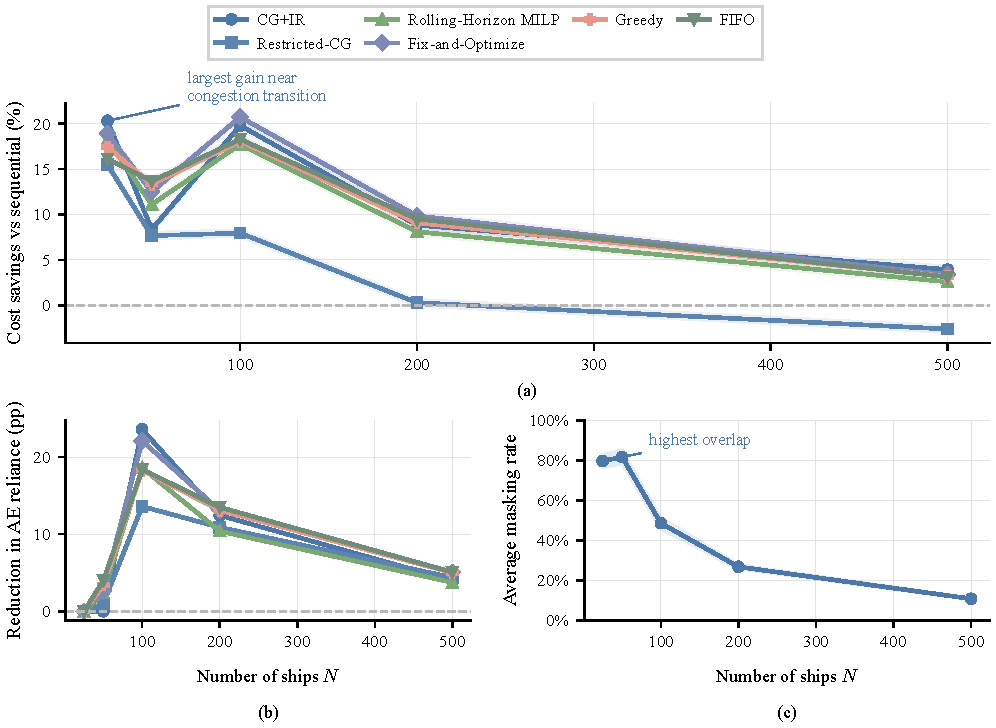
\includegraphics[width=0.98\textwidth]{figures_tr_style/pdf/Fig5_simops_insights.pdf}
    \caption{SIMOPS 主文图：不同方法下的降本幅度、停留时间变化，以及 CG 下的掩盖率分布和船型拆分结果。}
    \label{fig:simops_results}
\end{figure}

\paragraph{机制解释}
图 \ref{fig:simops_results} 的左下与右下面板进一步给出了掩盖效应的分布及其在船型间的差异。总体上，随着系统规模增大，掩盖率由 $N=25$ 时的 0.655 下降到 $N=500$ 时的 0.129，表明并行作业释放的时间收益会在高拥挤条件下被资源竞争逐步吞噬。结合第 \ref{sec:sensitivity} 节的敏感性分析可以看出，SIMOPS 的收益需要与基础设施容量相匹配；在容量不足时，并行化本身并不能替代资源扩容。

\FloatBarrier
\subsection{敏感性分析与管理启示}
\label{sec:sensitivity}
图 \ref{fig:sensitivity_results} 总结了关键参数的敏感性结果（$N=100$，U 场景）。首先，当电池成本由 0.30 增至 0.80 \$/kWh 时，系统总成本均值由 125287.86 上升至 318703.75，说明换电价格是决定系统经济性的关键参数；但在当前区间内，服务模式结构几乎保持不变，岸电占比稳定在约 0.149、换电占比稳定在约 0.851，仅在 0.80 \$/kWh 时出现极少量褐色模式（0.004）。这说明电池成本上升主要抬升了成本水平，但尚未触发大规模的模式切换。

其次，岸电容量扩张对成本和服务结构的影响更加直接。当岸电桩数量由 1 增至 8 时，平均总成本由 198105.48 下降至 133257.40，累计降幅约为 32.73\%；与此同时，岸电占比由 0.086 持续提升至 0.484，褐色模式占比由 0.032 降至 0。相比之下，截止期紧迫度的影响相对温和：当紧迫度系数由 0.80 提升至 1.20 时，平均成本仅由 185002.17 小幅降至 182638.89，但换电占比由 0.840 上升到 0.862，表明更宽松的时间窗口有助于提高绿色服务的可调度性，不过其边际作用弱于基础设施扩容。

\begin{figure}[!htbp]
    \centering
    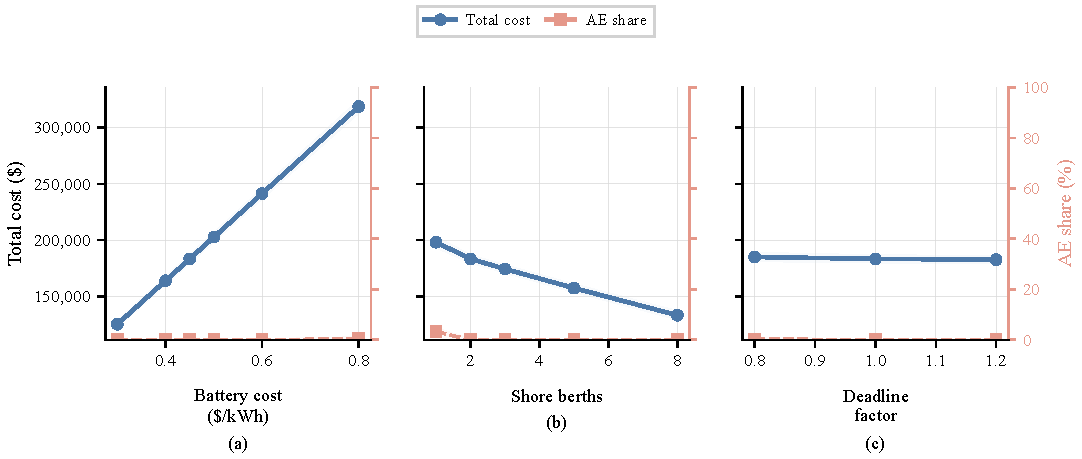
\includegraphics[width=0.98\textwidth]{figures_tr_style/pdf/Fig6_sensitivity.pdf}
    \caption{敏感性主文图：电池成本、岸电容量与截止期紧迫度对系统目标值及褐色模式占比的影响。}
    \label{fig:sensitivity_results}
\end{figure}

\FloatBarrier

\subsection{服务机制对比：混合补能的价值}
\label{sec:mechanism_comparison}
除场景和参数扰动外，本文进一步比较了三种服务机制：仅换电（battery-only）、仅岸电（shore-only）和混合补能（hybrid）。结果显示，混合机制在成本与可行性上均优于任何单一补能方案。以 CG 为例，hybrid 的平均总成本为 183337.84，明显低于 battery-only 的 217571.42 和 shore-only 的 357065.41；相应地，hybrid 相对 battery-only 与 shore-only 的平均降本幅度分别约为 15.73\% 和 48.65\%。这一结果说明岸电与换电并非简单替代关系，而是典型的互补关系：岸电提供低成本但服务时间较长的固定服务，换电提供高时效但成本较高的灵活服务，二者联合后能够在成本与可行性之间取得更优平衡。

从模式结构看，battery-only 机制下系统主要依赖换电，平均换电占比达到 0.896，但仍有 10.4\% 的需求落入褐色模式；shore-only 机制由于缺乏灵活补能手段，褐色模式占比高达 0.876；hybrid 机制则在岸电占比 0.149 与换电占比 0.851 之间形成分工，并将褐色模式压缩至 0。换言之，混合机制不仅降低了总成本，也显著提升了绿色服务覆盖率。该结论可由图 \ref{fig:scenario_mechanism} 的右侧面板进一步直观看出。

\FloatBarrier

\subsection{可扩展性与消融实验}
\label{sec:ablation}
为检验 CG 关键策略的作用，对 warm-start、稳定化与多列定价等变体进行消融。图 \ref{fig:ablation} 显示，不同 CG 变体在当前实例族上的目标值基本一致，平均目标值均约为 529465.00；运行时间也集中在 18.2s 左右，差异很小。这说明在本文实验规模与参数设定下，列生成主框架本身已足以支撑稳定求解，warm-start、稳定化与多列定价的额外收益更多体现在稳健性而非平均性能提升上。因此，这部分结果更适合作为方法稳健性的补充说明，而非正文中的主要贡献来源。

\begin{figure}[htbp]
    \centering
    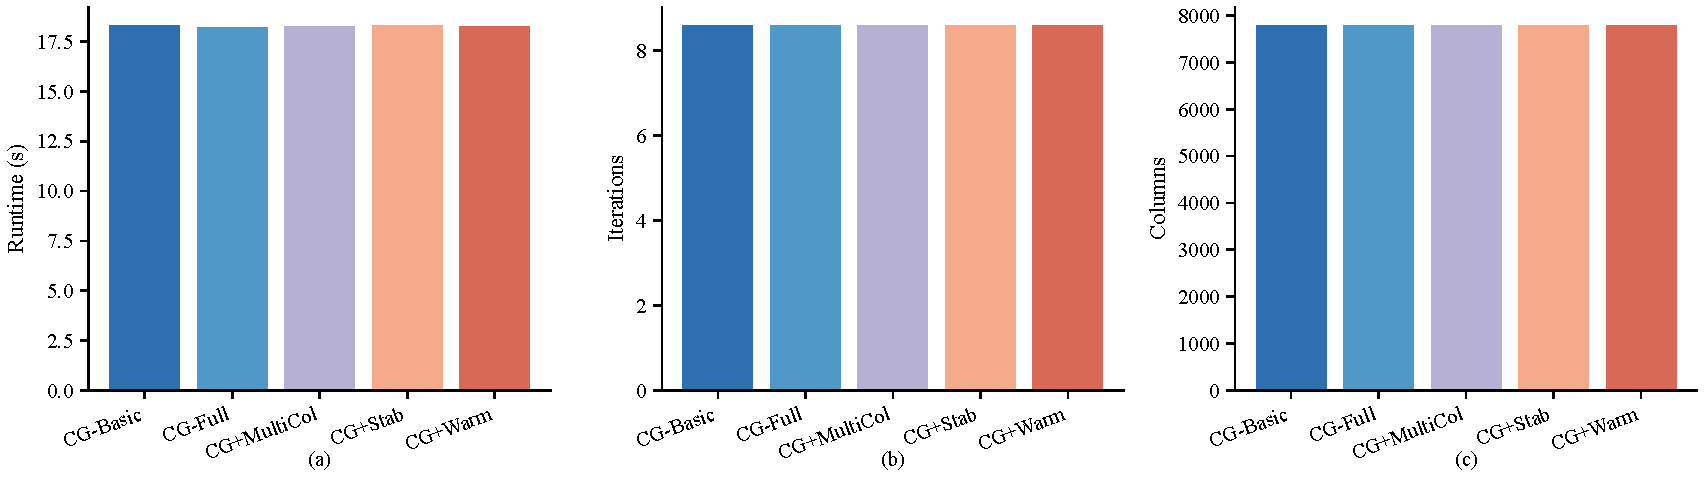
\includegraphics[width=0.98\textwidth]{figs/paper/Fig_Paper_Ablation.pdf}
    \caption{消融主文图：不同 CG 变体在运行时间、迭代次数与生成列数上的对比。}
    \label{fig:ablation}
\end{figure}

%% ================================================
%% 第四章：结论
%% ================================================

\section{结论}
\label{sec:conclusion}

\subsection{主要结论与机制解释}
\label{sec:main_findings}

本文围绕“异质船舶 + 异质补能方式 + SIMOPS 并行作业”这一组合调度问题，得到以下几个更稳健的结论。第一，CG 在当前实验组中始终保持最优的平均解质量，并在可有效验证的实例上与精确基准一致。具体而言，$N=20$ 和 $N=50$ 时 CG 与 MILP300 完全对齐；当规模增至 $N=100$ 时，限时 MILP 已难以稳定提供可靠基准，而 CG 仍保持 100\% 成功率；当规模增至 $N=200$ 和 $N=500$ 时，在扩大迭代预算后，CG 的平均目标值分别达到 535891.97 和 1690831.88，仍显著优于 Rolling-Horizon、Fix-and-Optimize、Restricted-CG、FIFO 和 Greedy。

第二，不同算法家族体现出清晰的功能分工。Rolling-Horizon 代表滚动近似优化，具有较好的工程可实施性，但受窗口提交机制影响，其全局协调能力受限；Fix-and-Optimize 代表局部精确改进，在解质量上整体强于 Rolling-Horizon，但仍明显弱于完整 CG；Restricted-CG 代表快速近似列生成，运行速度极快，但解质量损失最为明显。这说明本文方法的优势并非建立在与简单启发式的对比之上，而是在与多类代表性近似优化框架的比较中依然成立。

第三，SIMOPS 的价值是条件性的，而非无条件单调的。实验表明，SIMOPS 在 $N=25,50,100$ 时分别带来 20.29\%、8.37\% 和 19.71\% 的平均降本，但在 $N=200$ 和 $N=500$ 时相对串行作业反而出现 0.45\% 和 0.90\% 的小幅成本反转，说明并行作业的收益需要与基础设施能力相匹配。当系统负载超过一定阈值后，资源竞争会吞噬掩盖效应带来的时间优势。

第四，到达过程的集中性比作业时长整体拉长更容易触发系统性拥堵。在三类场景中，峰值到达场景（P）的系统成本最高，且 CG 相对 FIFO 和 Greedy 的改进幅度也最大。这意味着港口能否平滑吸收到港高峰，是决定系统总成本和绿色服务绩效的关键因素之一。

第五，混合补能机制与岸电扩容具有明确的结构性价值。hybrid 机制显著优于 battery-only 与 shore-only，说明岸电与换电本质上是互补而非替代关系；同时，敏感性分析表明岸电容量扩张相较单纯的价格调节更能实质性改变服务模式结构，从而在降低总成本的同时提升绿色服务覆盖率。

\subsection{方法贡献与管理含义}
\label{sec:contributions}

在方法层面，本文的首要贡献在于将 SIMOPS 从工程操作规则转化为可优化约束。与既有串行作业模型相比\cite{Dai2020,Zou2024}，离港时间不再由“装卸完成后再补能”的线性结构决定，而由 $L_i=\max\{\text{cargo finish},\text{service finish}\}$ 的并行结构决定，从而能够显式刻画装卸与能源服务之间的时间重叠。修正后的实验结果进一步表明，这一结构不是简单导向“并行总是更优”，而是揭示了 SIMOPS 收益与容量条件之间的内在关系，这使模型的解释力更接近真实港口运行机制。

本文的第二项贡献在于统一刻画固定岸电、移动换电与燃油辅机三类服务，在同一框架下识别成本、时效与可行性的三重权衡。结果表明，混合补能机制稳定优于任何单一机制，这意味着港口能源转型不应被理解为“单一技术替代”，而应被理解为异质资源之间的组合优化问题。燃油辅机在模型中并非鼓励使用，而是作为可行性兜底选项存在，其高成本设定确保只有在绿色方案不可行或代价过高时才被激活。

在算法层面，本文不仅提出了完整 CG 框架，还通过 Rolling-Horizon、Fix-and-Optimize 和 Restricted-CG 三类新增基线，系统对比了不同近似优化哲学。结果表明，Rolling-Horizon 牺牲了全局协调能力，Fix-and-Optimize 受限于局部邻域改进，Restricted-CG 则通过限制定价范围换取了极高速度；相比之下，完整 CG 在可校准性、解质量和大规模鲁棒性之间提供了更优平衡。因此，本文的贡献不只是“提出了一个更快的方法”，而是给出了一个在 tractable instances 上可验证、在 large-scale instances 上仍具竞争力的统一求解框架。

在管理层面，本文结果支持“先优化协同，再定向扩容”的实施路径。对于运营管理者而言，SIMOPS 只有在岸电和换电能力足以支撑并行需求时才会稳定带来收益；对于投资规划者而言，扩充岸电容量比单纯调整价格参数更能形成结构性改善，因为它不仅降低总成本，还会直接提高绿色服务占比并减少褐色模式使用。因此，港口更合理的实践路径是：以混合补能机制为基础，在中等负载或高时敏业务上优先部署 SIMOPS，并将新增投资重点放在已识别的容量瓶颈上。

\subsection{局限、拓展方向与结语}
\label{sec:limitations}

本文仍存在若干局限。首先，研究采用确定性到达与需求设定，而现实中船期偏差、作业扰动与负荷波动普遍存在\cite{UNCTAD2021}；随机或鲁棒优化能够提升抗扰性，但也会显著增加计算负担\cite{Rodrigues2022}。其次，当前框架以总成本最小化为单一目标，尚未显式纳入排放、公平与服务可靠性等多目标权衡。再次，泊位分配在本文中外生给定，尚未与能源调度联合优化，而泊位位置本身会影响岸电可用性与并行作业可实施性\cite{Dai2020}。最后，尽管扩大迭代预算后的 CG 已显著改善了大规模实例表现，但对更高负载情形而言，如何进一步设计自适应 stopping rule 与更强的列管理策略，仍是提升超大规模求解效率的重要方向。

基于上述局限，后续研究可以沿四个方向展开：其一，将可再生能源、港内储能与岸电调度联立建模，研究补能资源与电力侧灵活性的协同\cite{Li2022_BSS}；其二，在到达时间、负荷和电价存在不确定性的条件下，构建日前规划与实时重调度联动的两阶段模型；其三，利用学习方法辅助列生成中的热启动、列筛选与 stopping rule 设计，以提升超大规模实例下的在线性能\cite{Bengio2021}；其四，将移动换电单元扩展到多码头网络场景，研究码头间重定位与码头内调度之间的双层协调。

总体而言，本文的修正结果表明：SIMOPS 不是一个可以脱离容量条件单独讨论的操作细节，而是与基础设施能力、船舶异质性和服务机制共同决定系统成本边界的关键因素。只有在“并行作业机制 + 混合补能结构 + 可扩展优化方法”三者协同作用下，港口电气化转型才能同时兼顾经济性、可行性与绿色化目标。由此，本文提出的统一建模与求解框架，为港口绿色转型提供了一个更可解释、也更接近工程落地场景的分析基础。

\FloatBarrier

%% --- 参考文献区 ---
\bibliographystyle{plain} % 或者使用 gbt7714-numerical
\bibliography{ref11}

\end{document}
